
\documentclass[a4paper,12pt]{article}

\usepackage{graphicx}
\usepackage{a4wide}
\usepackage{adjustbox}
\usepackage{float}
\usepackage{lineno}
\usepackage{setspace}
  \doublespacing

\begin{document}

\Large
Appendix S2

AppendixS2.pdf

Comparison of large-scale citizen science data and long-term study data for phenology modeling

\normalsize
\textit{Shawn D. Taylor, Joan M. Meiners, Kristina Riemer, Michael C. Orr, Ethan P. White}

\textbf{\large Supplementary materials}

Supplementary images S1 - S11 and Tables S1-S2


%%%%%%%%%%%%%%%%%
%% Figure S1
%%%%%%%%%%%%%%%%%
\newpage

\textbf{Figure S1}: Sensitivity test results from using a 15 versus 30 day cutoff between the 'yes' and most recent 'no' in the USA-NPN dataset. Each point represents the value of a single parameter for one of eight models for 32 unique species/phenophase combinations. This is from 23 species with varying combinations of the budburst and flowering phenophases (see Table S1). Only 32 comparisons were possible here as the stricter 15 day cutoff resulted in three species/phenophase combinations not having sufficient observations. This figure does not include any data from the LTER datasets. Note that the primary analysis states 35 combinations using the 15 day cutoff. This is because 3 species are duplicated in the Harvard Forest and Hubbard Brook datasets, thus 3 extra comparisons are available for the primary analysis. 

\newpage

\begin{center}
	\centering
		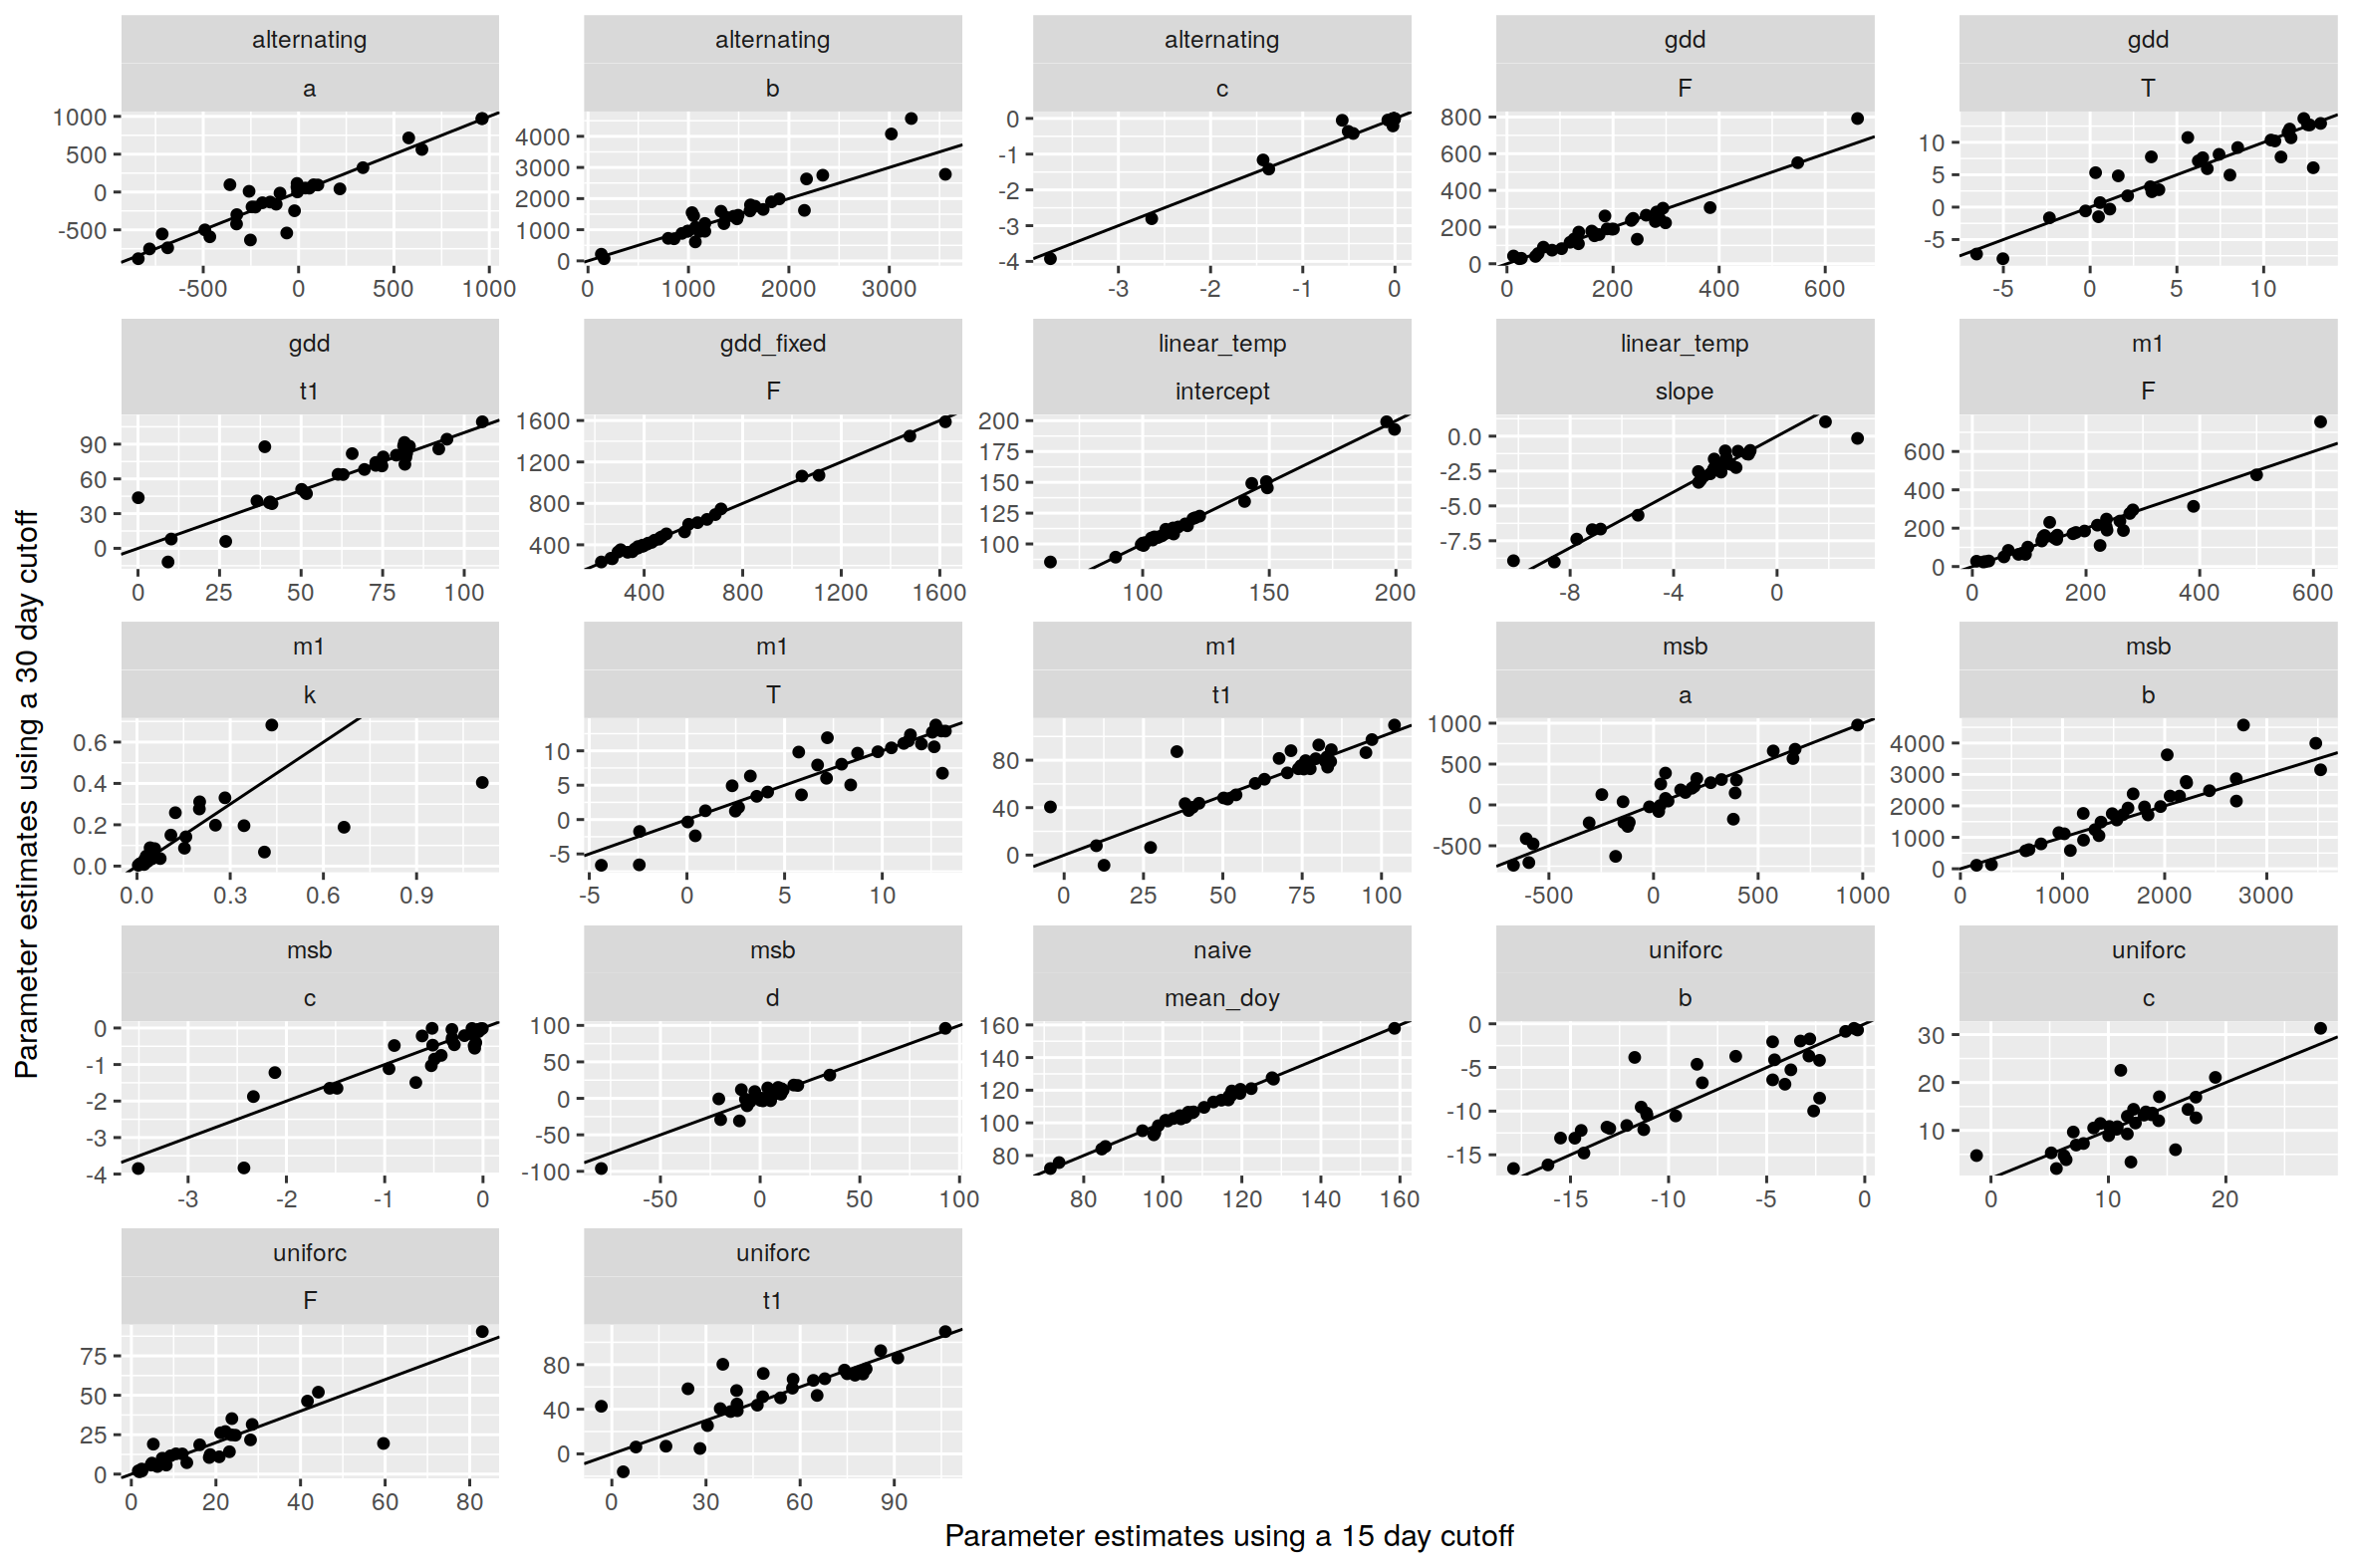
\includegraphics[width=1\textwidth]{figure_s1_parameter_estimates_from_cutoff_sensitivity.png}
	Figure S1
\end{center}

\newpage

%%%%%%%%%%%%%%%%%
%% Figure S2
%%%%%%%%%%%%%%%%%
\newpage

\textbf{Figure S2}: Comparisons of parameter estimates between NPN and LTER derived models. As in Figure 2 in the main text, but using a threshold of 15 instead of 30 days between the first 'yes' and most recent 'no' in the USA-NPN dataset. See methods for details. 

\newpage

\begin{center}
	\centering
		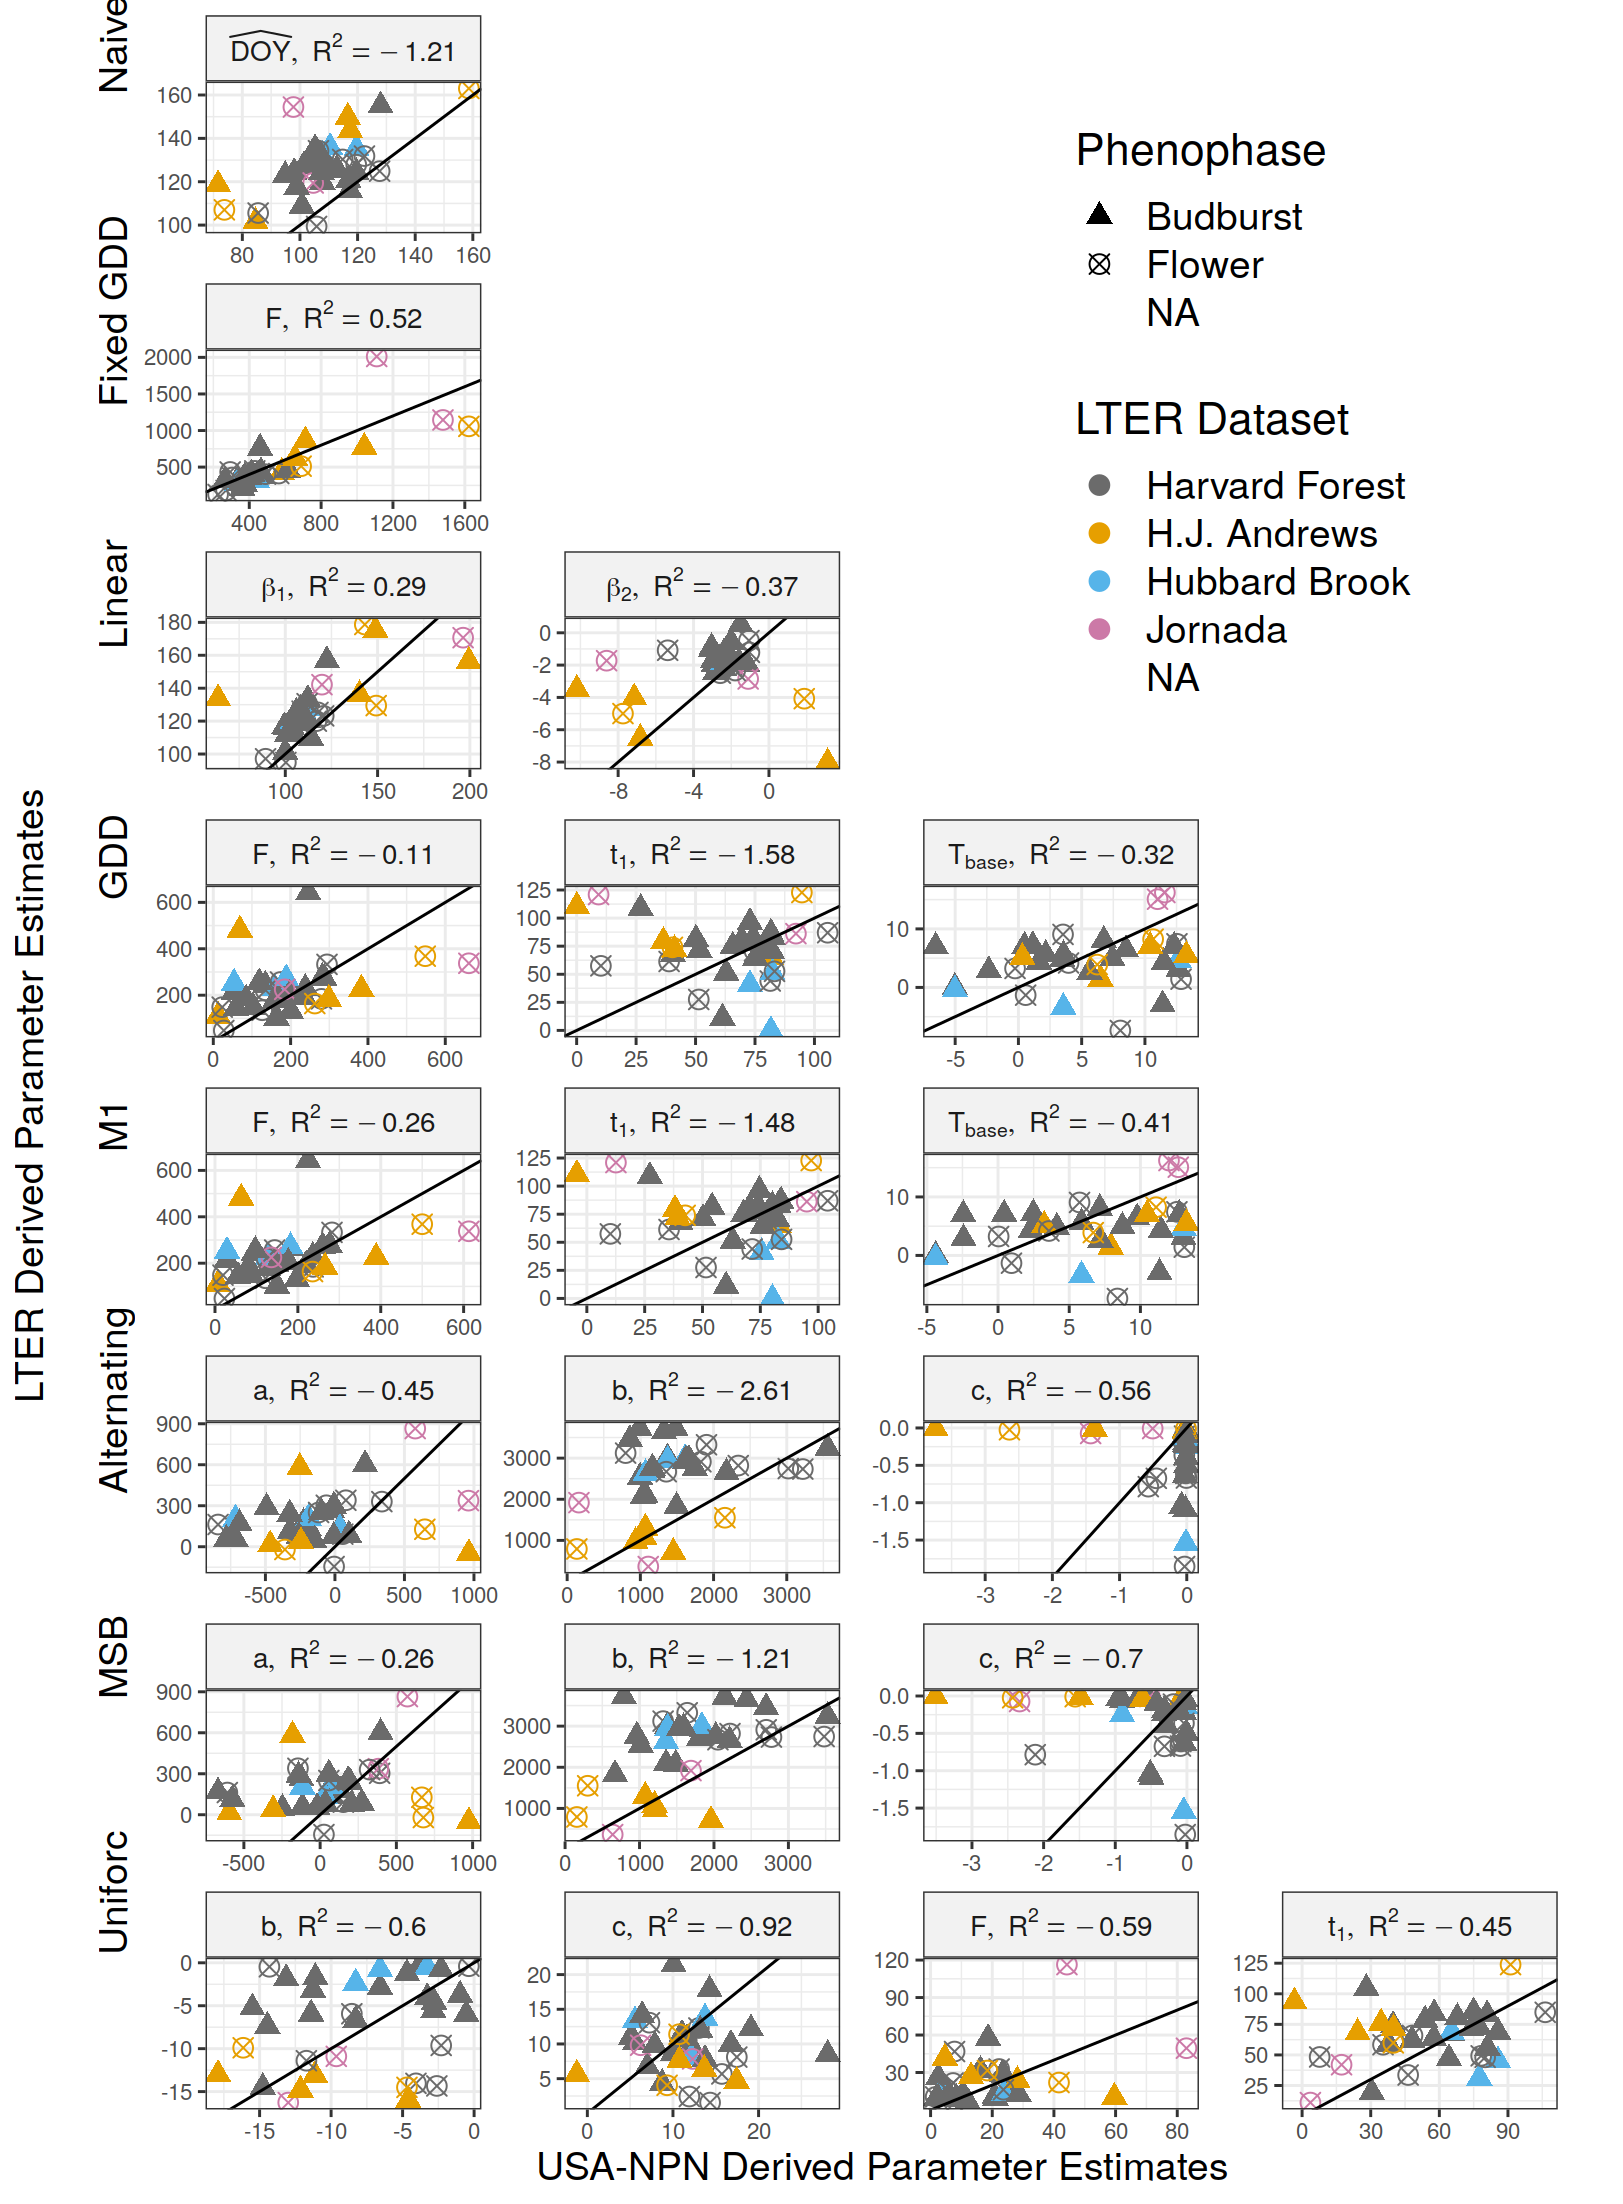
\includegraphics[scale=0.7]{figure_s2_param_comparison.png}
	Figure S2
\end{center}

\newpage

%%%%%%%%%%%%%%%%%
%% Figure S3
%%%%%%%%%%%%%%%%%
\newpage

\textbf{Figure S3}: Comparison of predicted day of year (DOY) of all phenological events between NPN
and LTER-derived models. As in Figure 3 in the main text, but using a threshold of 15 instead of 30 days between the first 'yes' and most recent 'no' in the USA-NPN dataset. See methods for details. 

\newpage

\begin{center}
	\centering
		\includegraphics[width=1\textwidth]{figure_s3_estimate_compare.png}
	Figure S3
\end{center}

\newpage

%%%%%%%%%%%%%%%%%
%% Figure S4
%%%%%%%%%%%%%%%%%
\newpage

\textbf{Figure S4}: Differences in prediction error between NPN and LTER-derived models. As in Figure 4 in the main text, but using a threshold of 15 instead of 30 days between the first 'yes' and most recent 'no' in the USA-NPN dataset. See methods for details. 

\newpage

\begin{center}
	\centering
		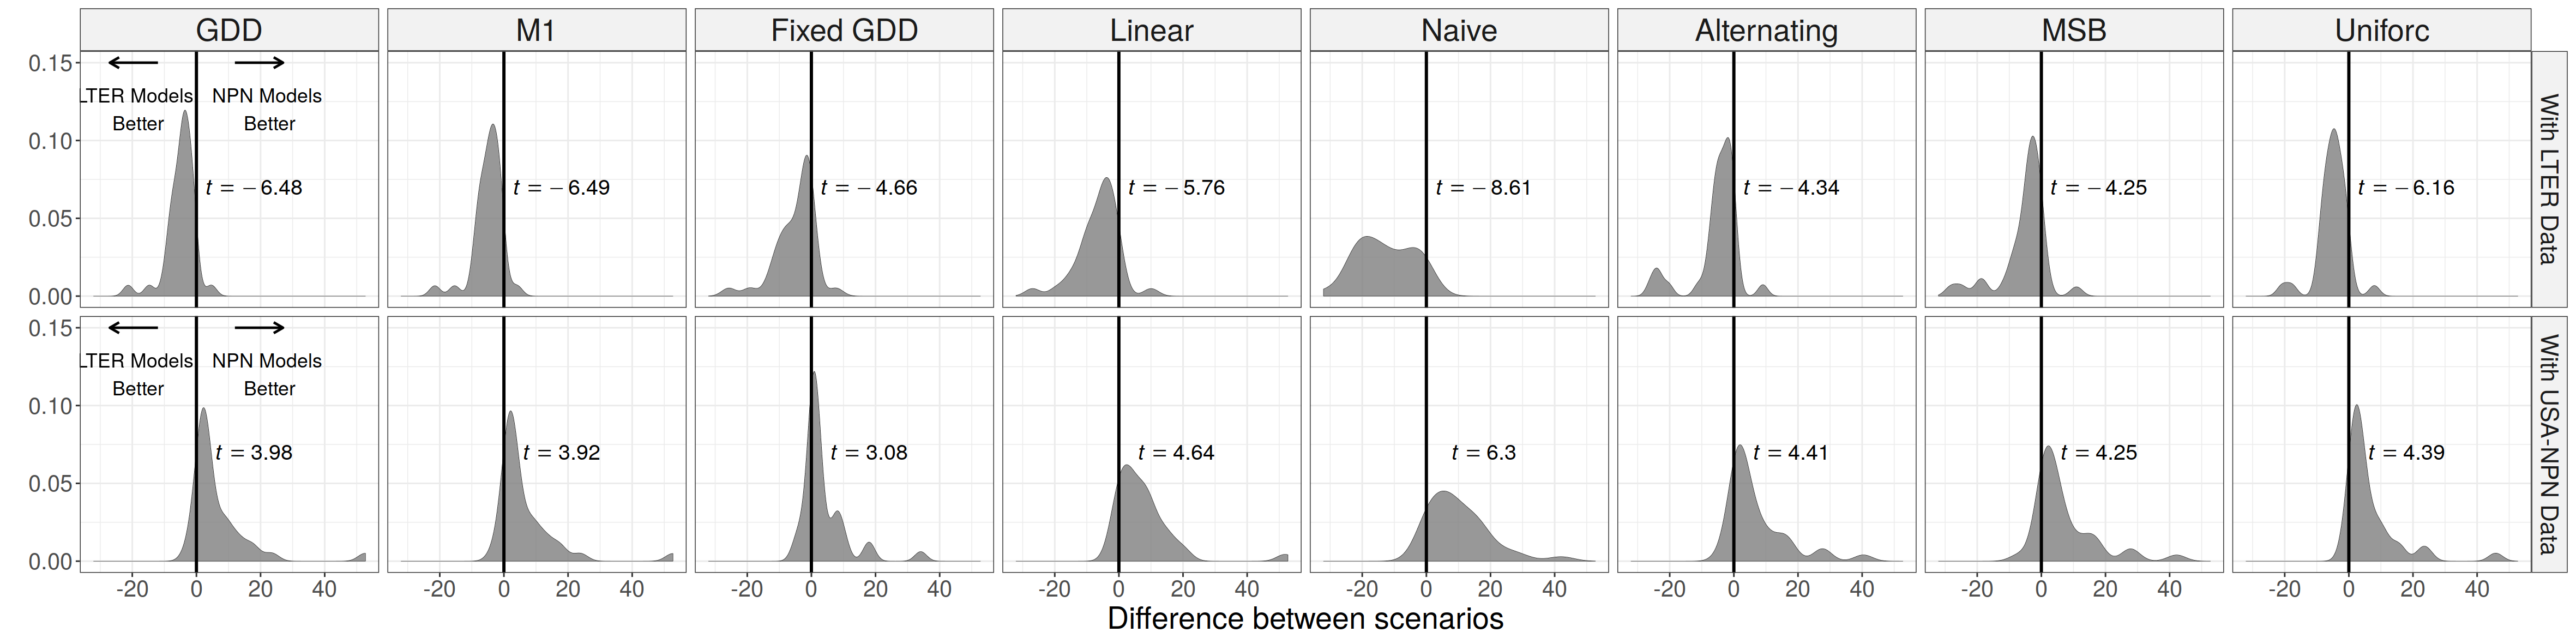
\includegraphics[width=1\textwidth]{figure_s4_rmse_metrics_density_plot.png}
	Figure S4
\end{center}

\newpage

%%%%%%%%%%%%%%%%%
%% Figure S5
%%%%%%%%%%%%%%%%%
\newpage

\textbf{Figure S5}: RMSE for specific species and phenophases using all combinations of models and data sources. Red X's mark the best performing models for each respective dataset. 

\newpage

\begin{center}
	\centering
		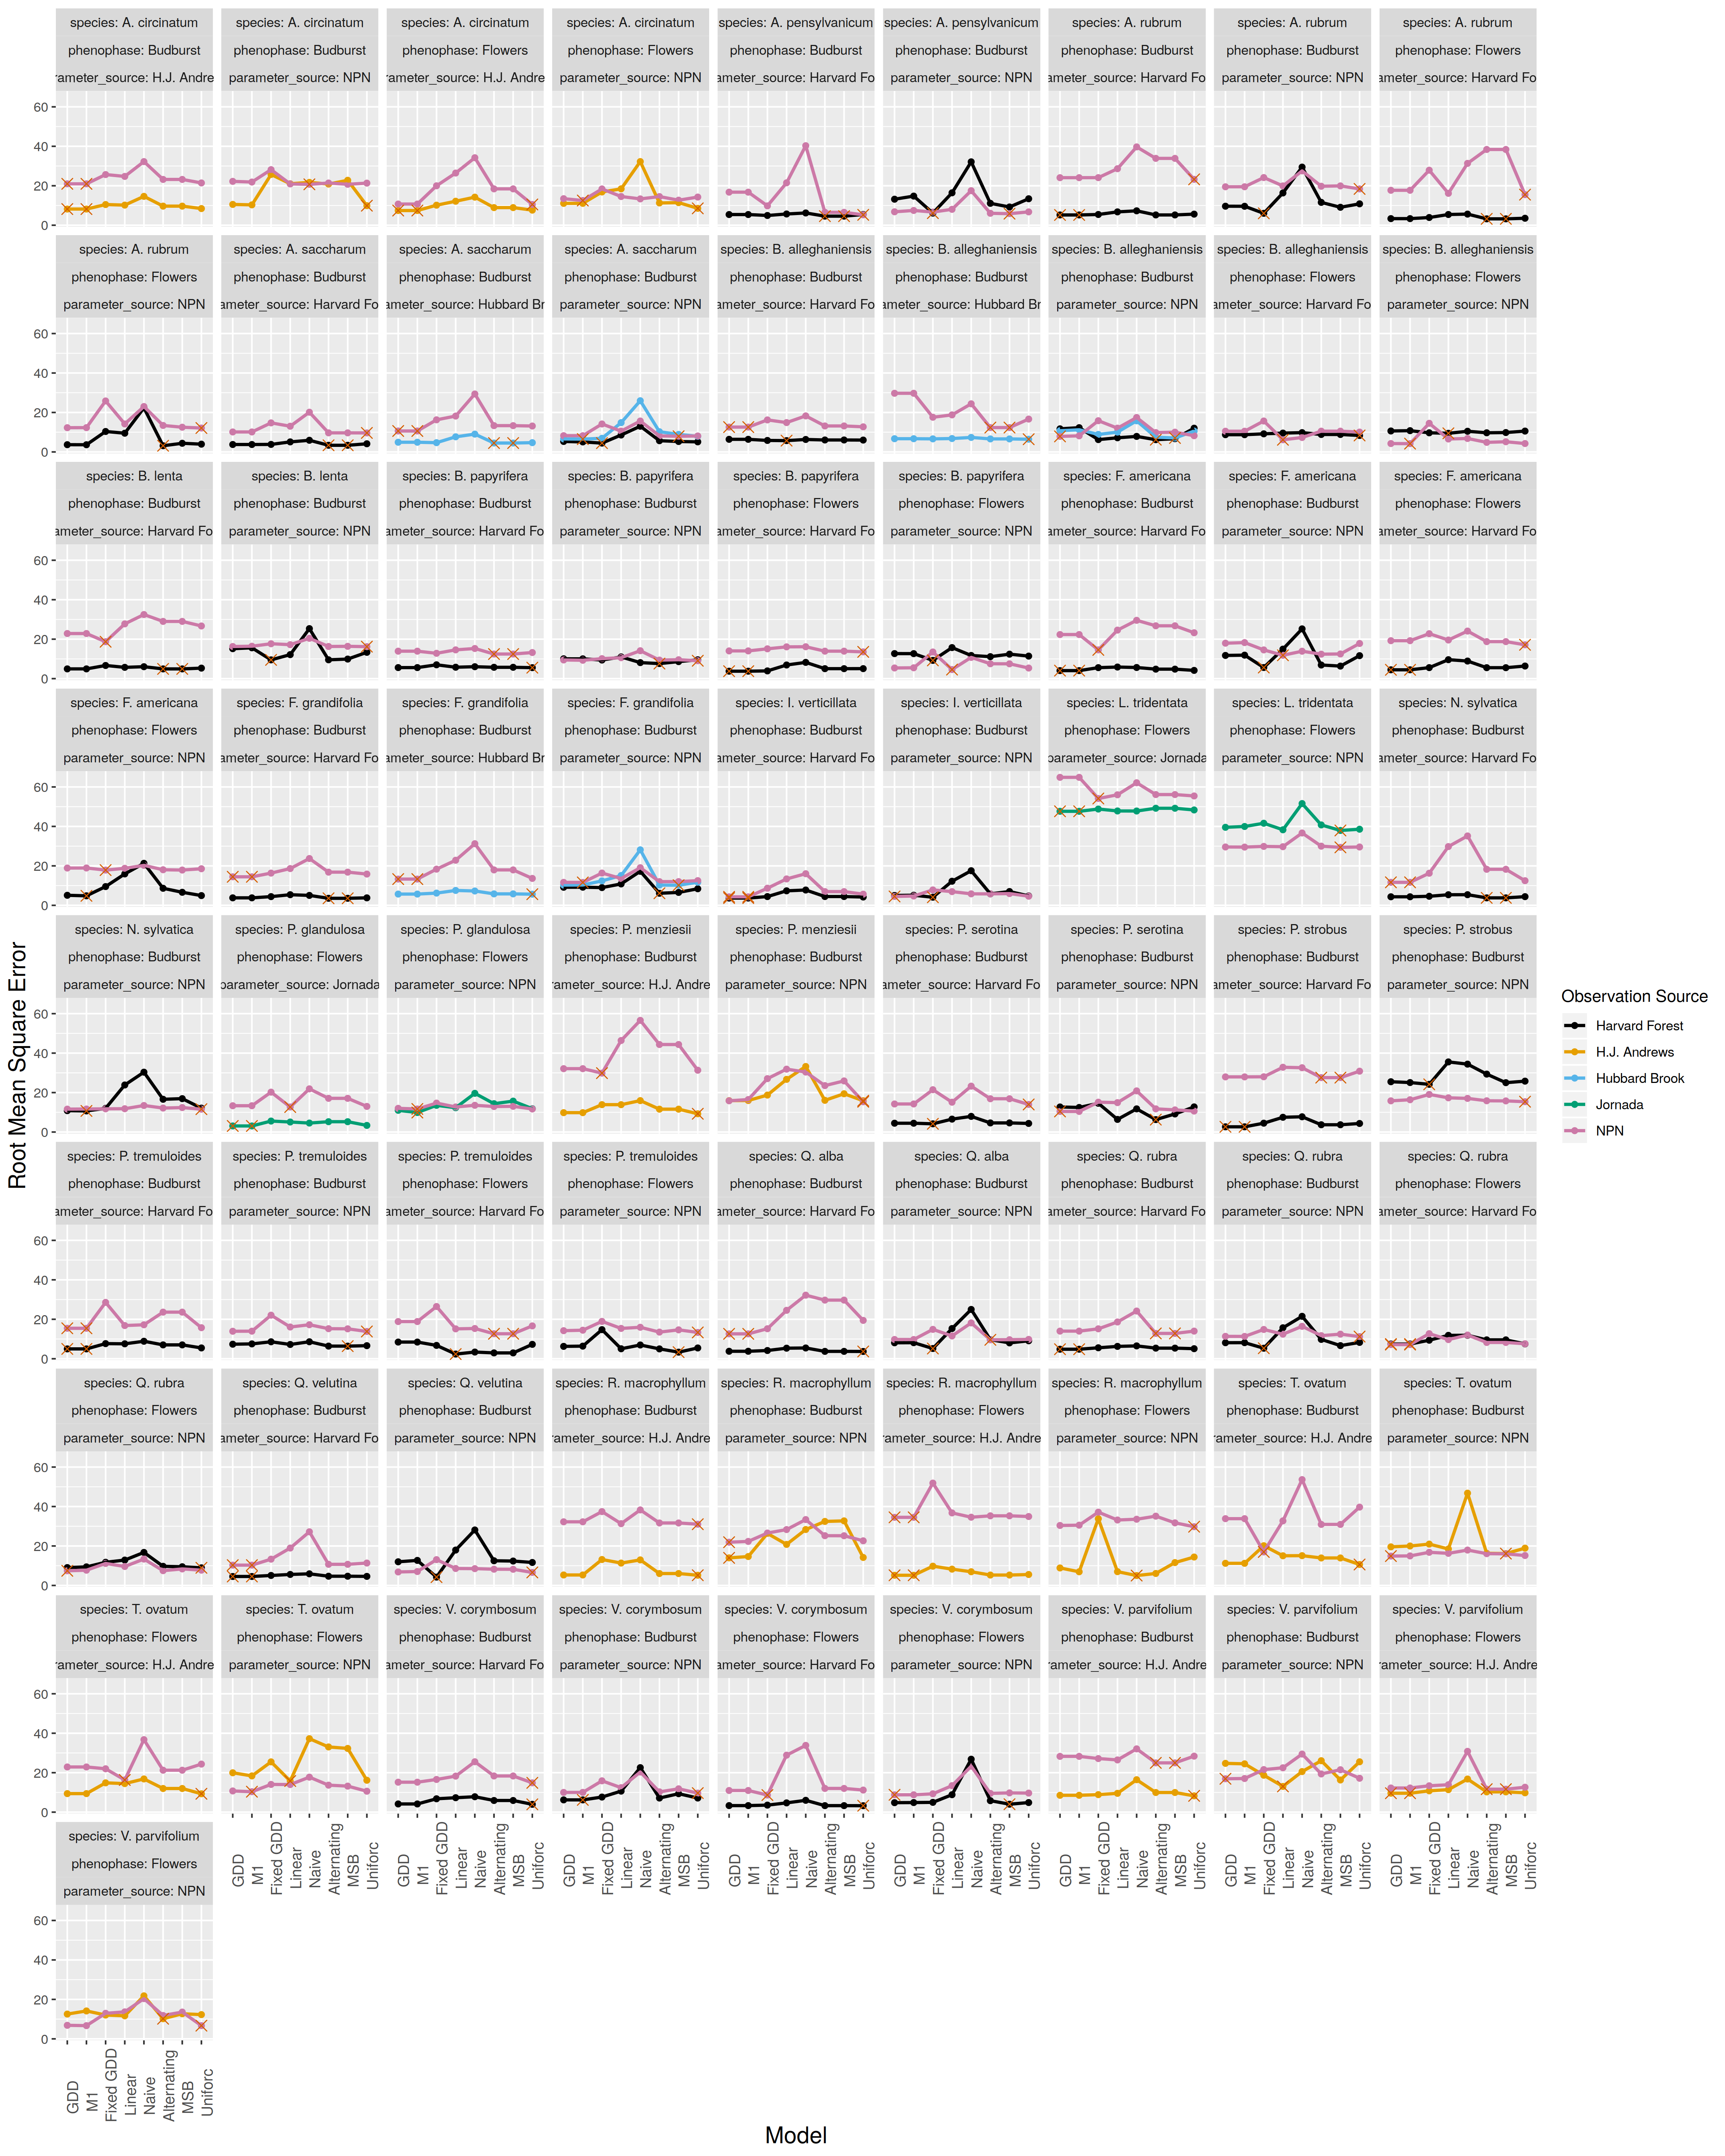
\includegraphics[width=1\textwidth]{figure_s5_all_model_rmse.png}
	Figure S5
\end{center}

\newpage
%%%%%%%%%%%%%%%%%
%% Figure S6
%%%%%%%%%%%%%%%%%
\textbf{Figure S6}: Pearson correlation coefficients for specific species and phenophases using all combinations of models and data sources. Note that since all predictions from each Naive model are the same the Pearsons correlation cannot be calculated here. Red X's mark the best performing models for each respective dataset.

\newpage

\begin{center}
	\centering
		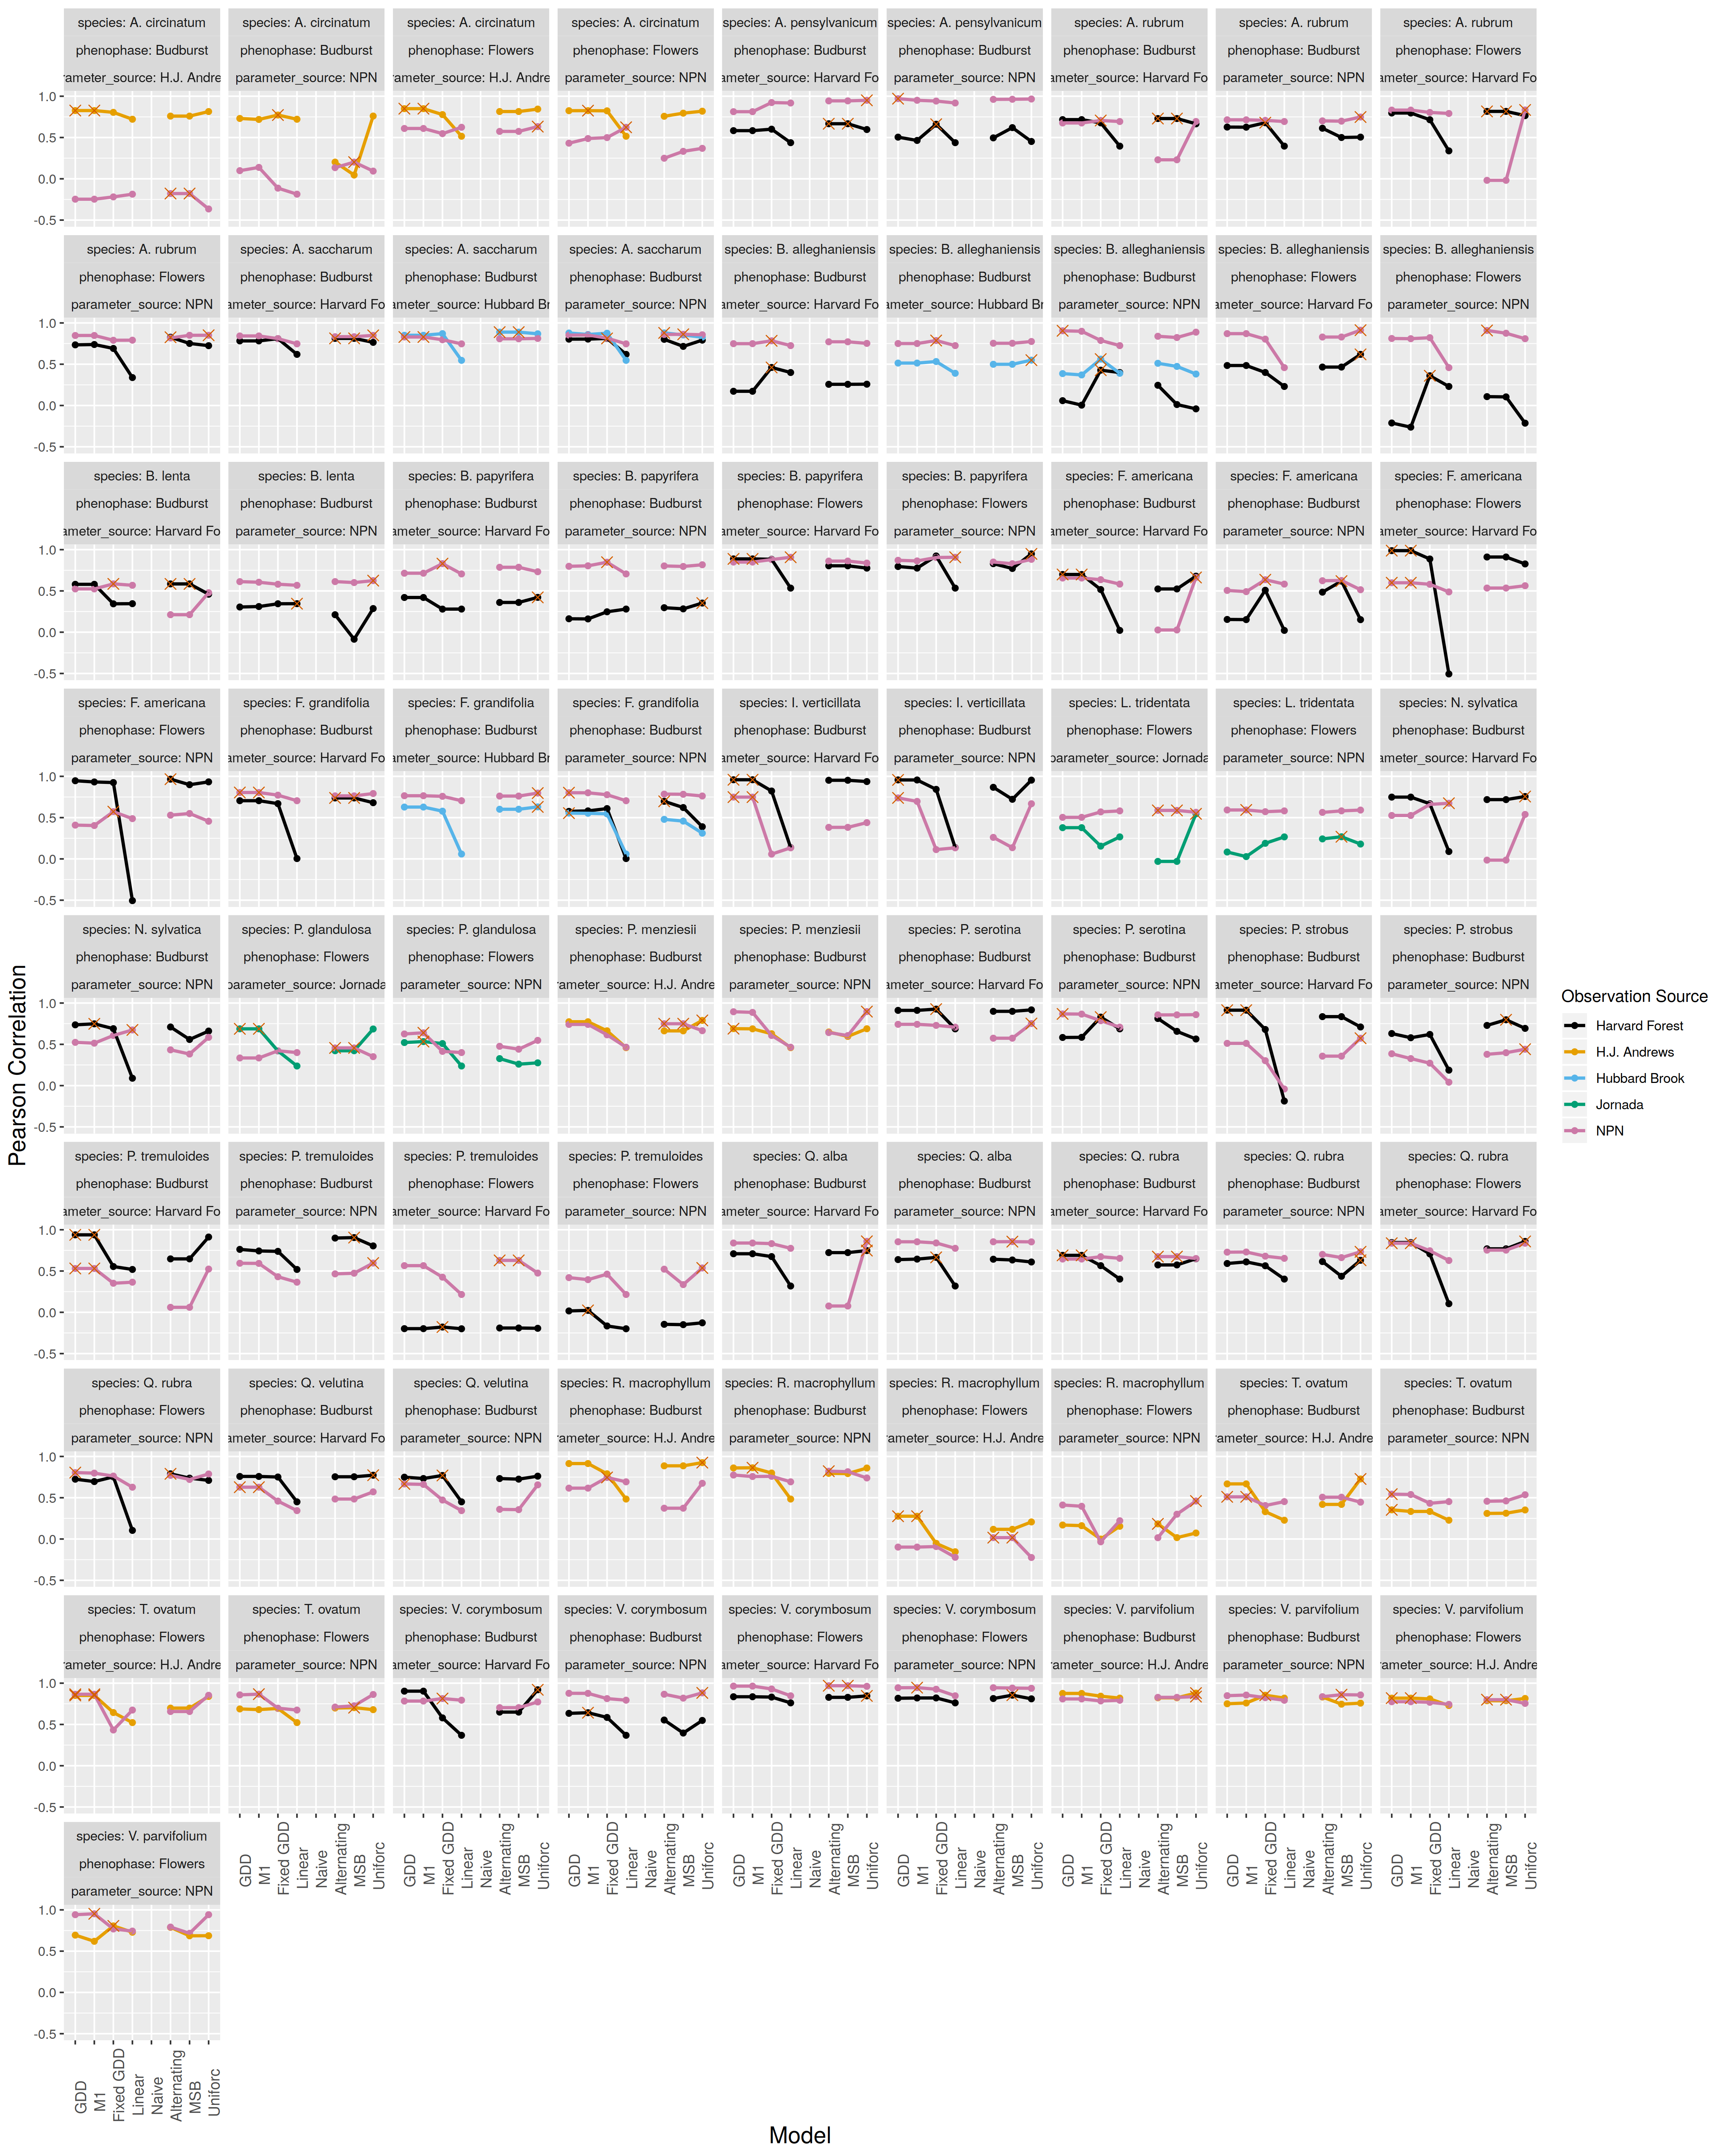
\includegraphics[width=1\textwidth]{figure_s6_all_model_pearson.png}
	Figure S6
\end{center}

%%%%%%%%%%%%%%%%%
%% Figure S7
%%%%%%%%%%%%%%%%%

\newpage

\textbf{Figure S7}: RMSE of all species and phenophases of the four scenarios described in the text. These values were calculated using held out test data.

\newpage

\begin{center}
	\centering
		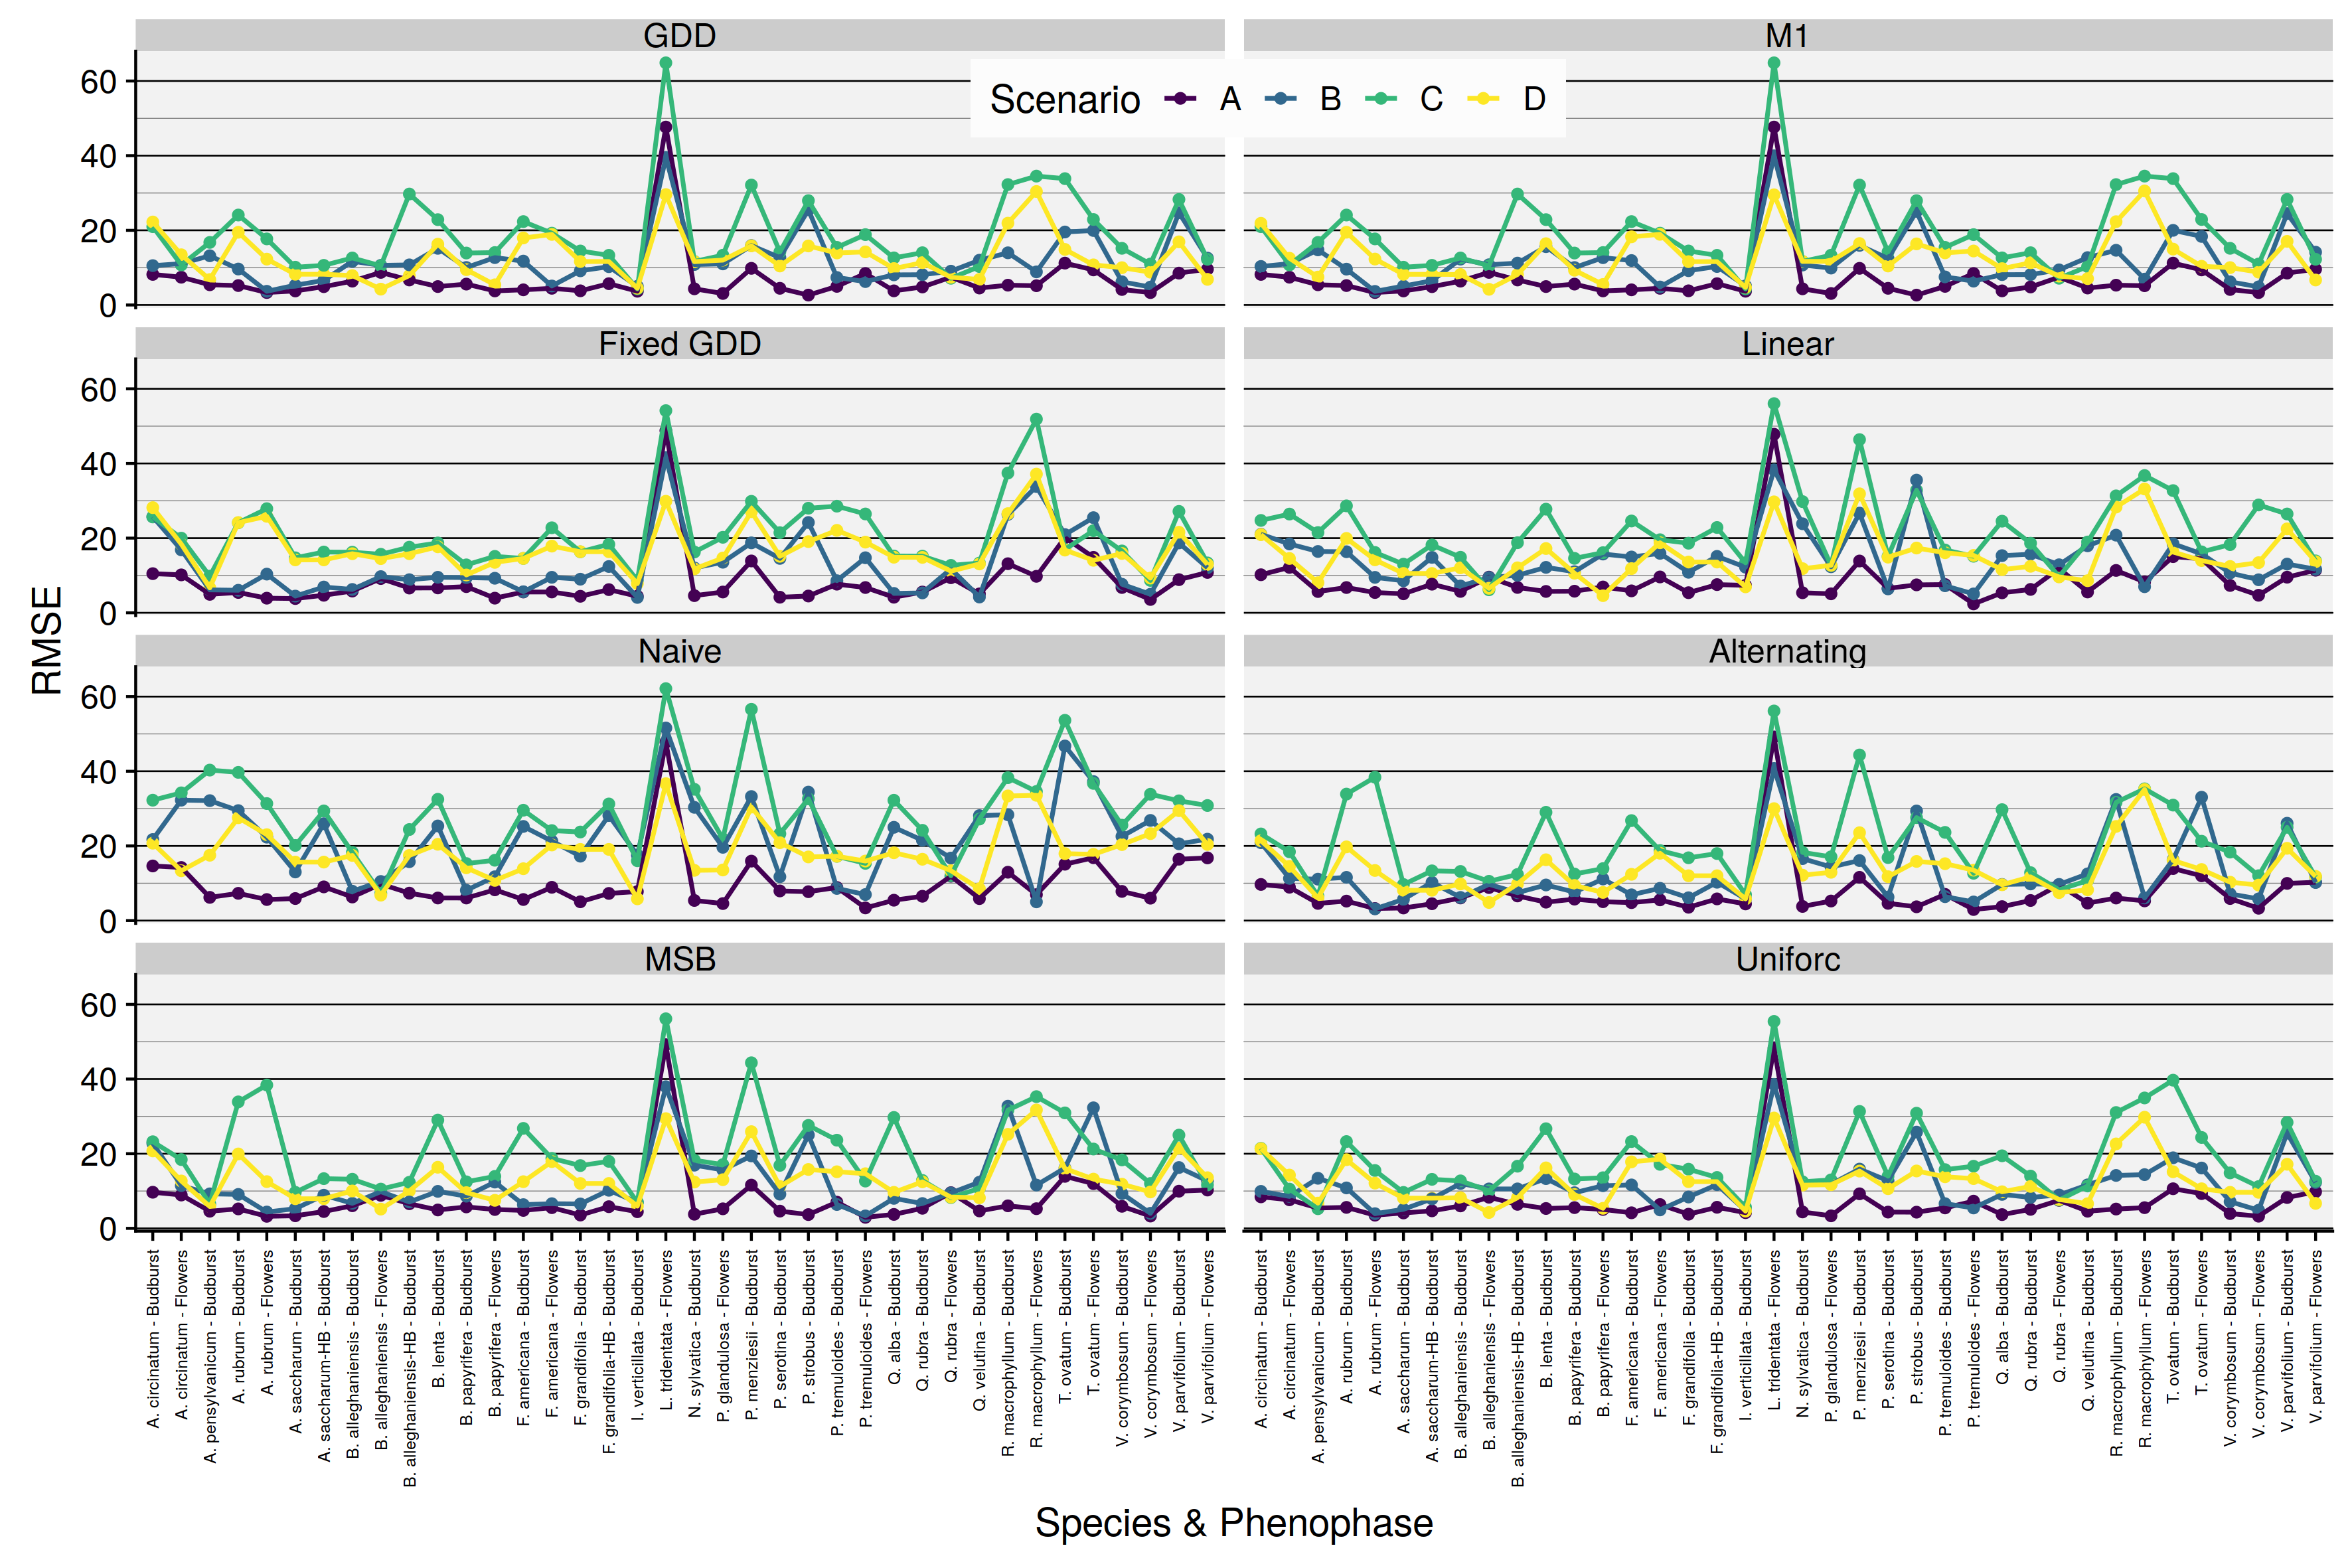
\includegraphics[width=1\textwidth]{figure_s7_scenario_absolute_rmse.png}
	Figure S7
\end{center}

%%%%%%%%%%%%%%%%%
%% Figure S8
%%%%%%%%%%%%%%%%%
\newpage

\textbf{Figure S8}: Distribution of parameters of the Naive, GDD, Fixed GDD, and Linear models for the three species common to the Hubbard Brook, Harvard, and USA-NPN datasets. The phenophase is budburst for all three species. Vertical lines indicate either the mean (solid) or median (dashed) of the respective distribution. Note the heading for each sub figure. 

\newpage

\begin{center}
	\centering
		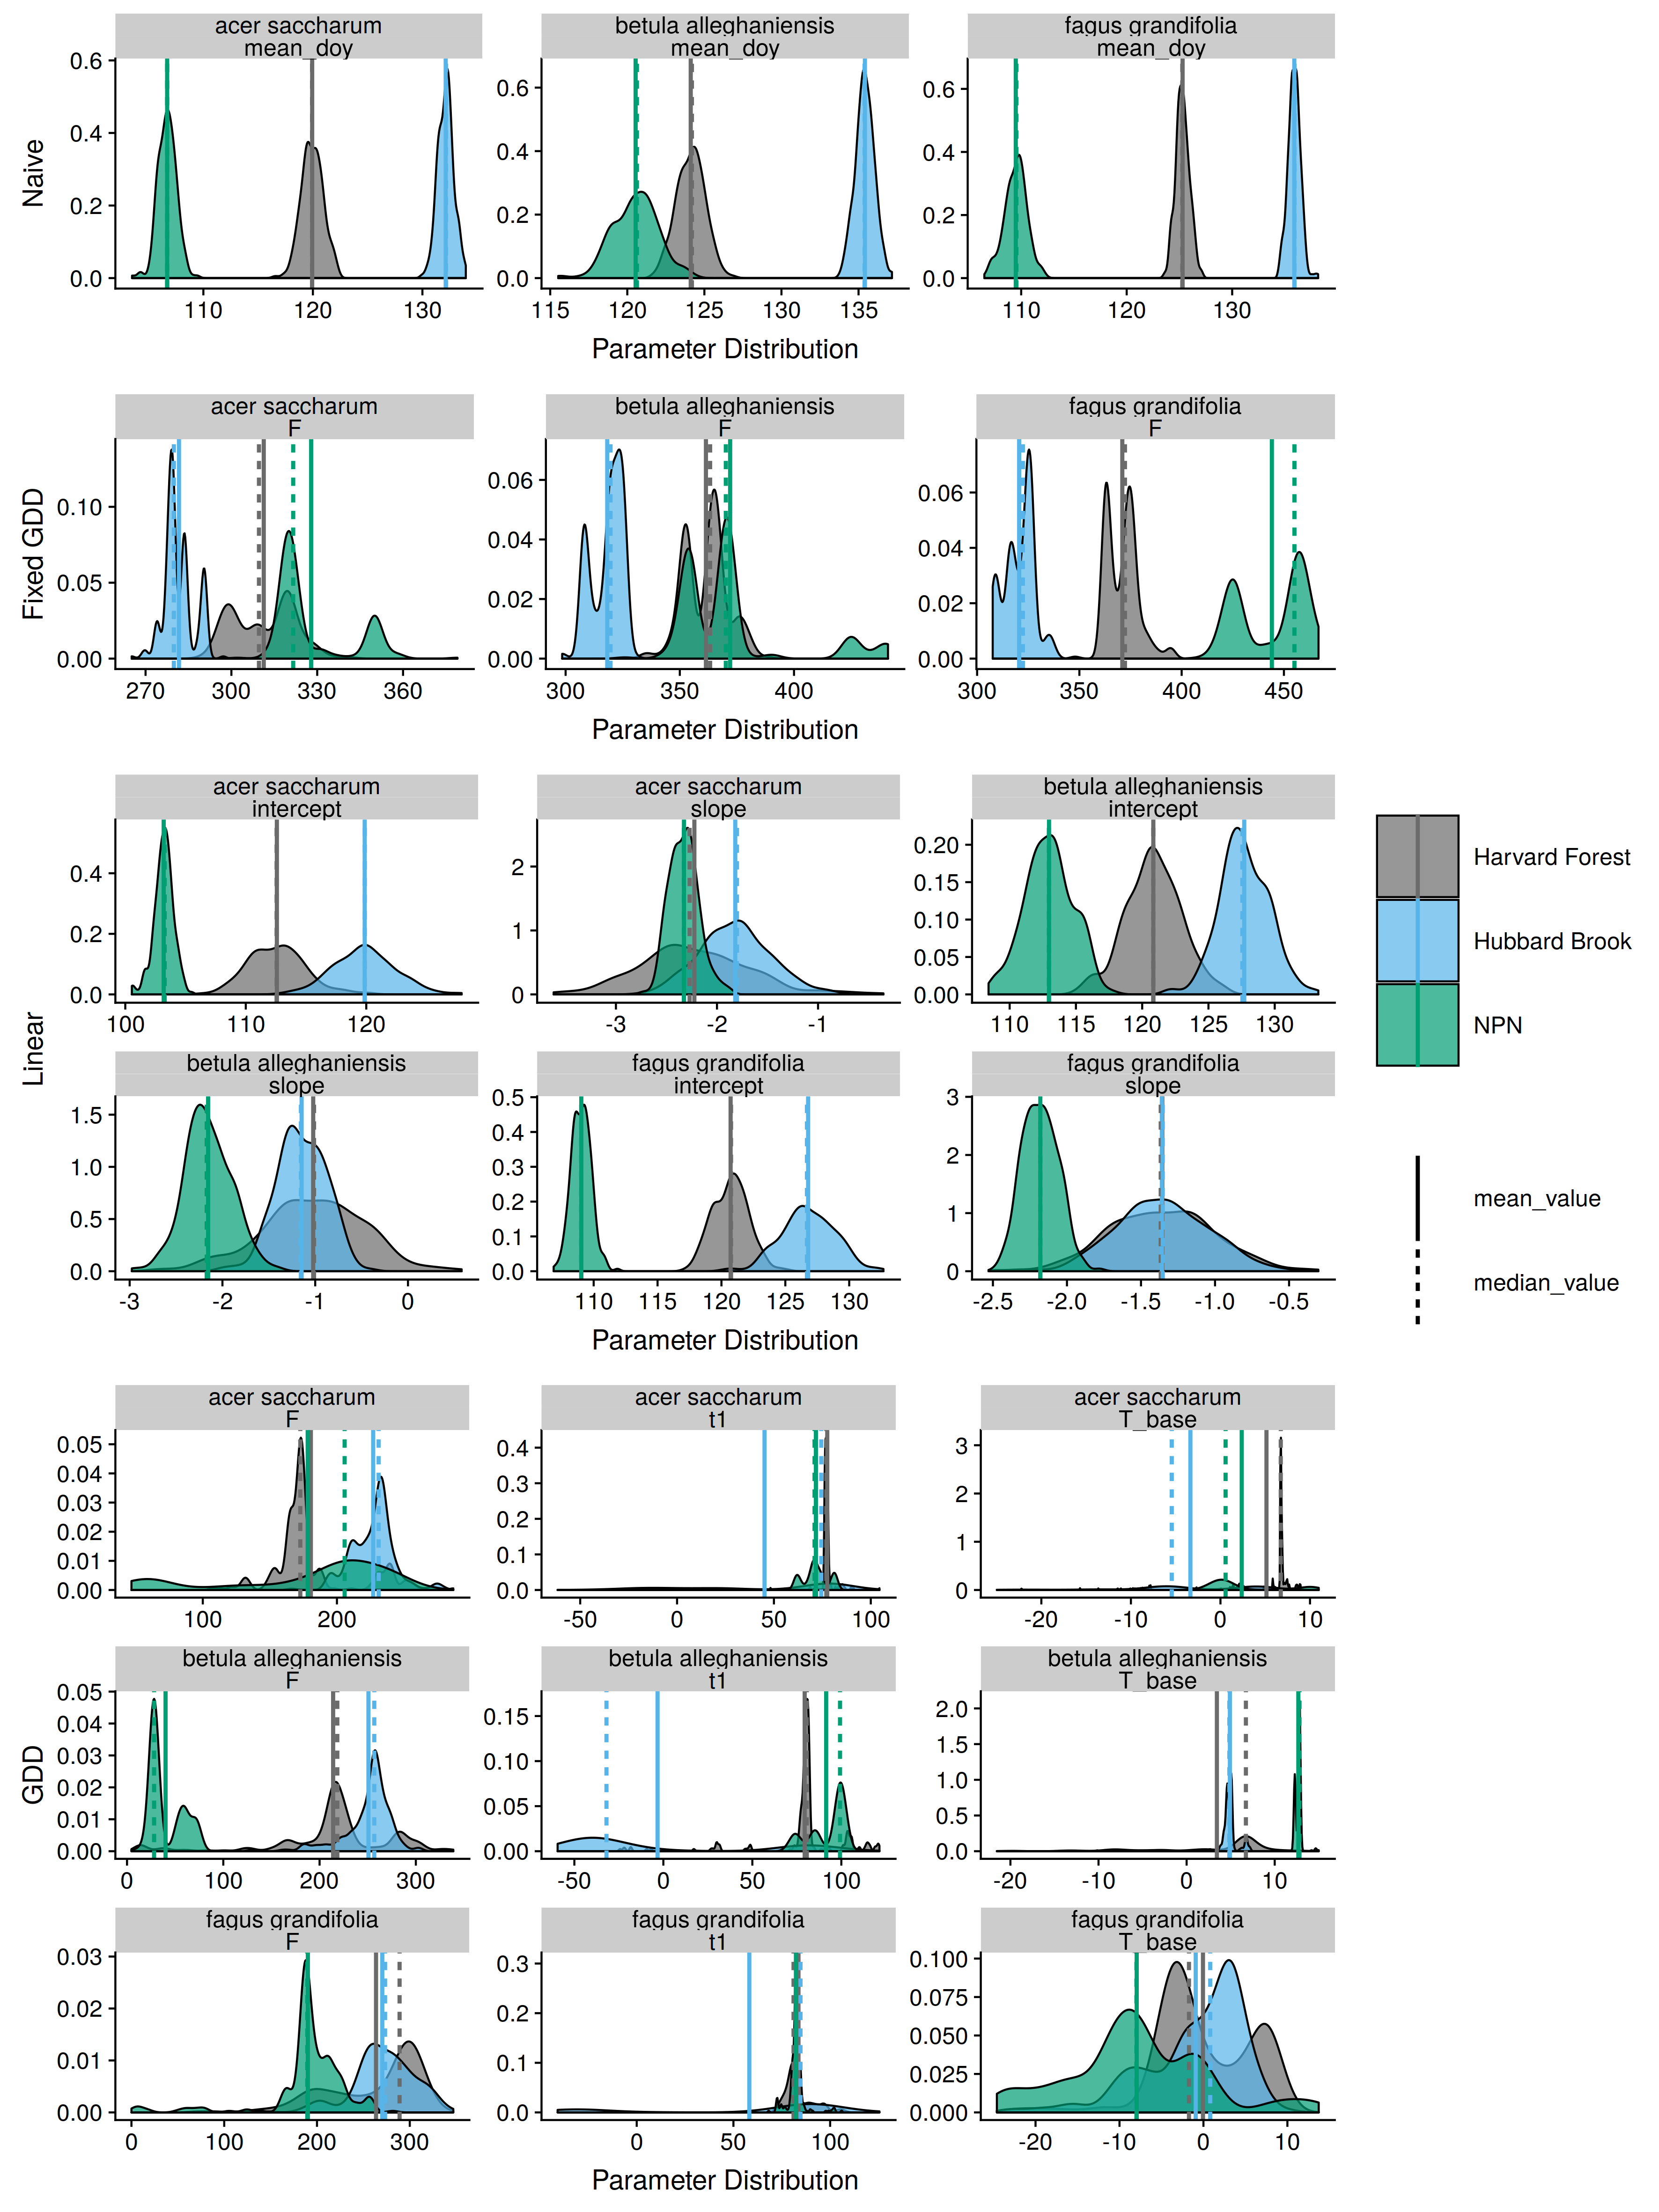
\includegraphics[scale=0.5]{figure_s8_hubbard_harvard_comparison1.png}
	Figure S8
\end{center}

%%%%%%%%%%%%%%%%%
%% Figure S9
%%%%%%%%%%%%%%%%%
\newpage

\textbf{Figure S9}: As in Figure S4, but for the Alternating and Uniforc models. 

\newpage

\begin{center}
	\centering
		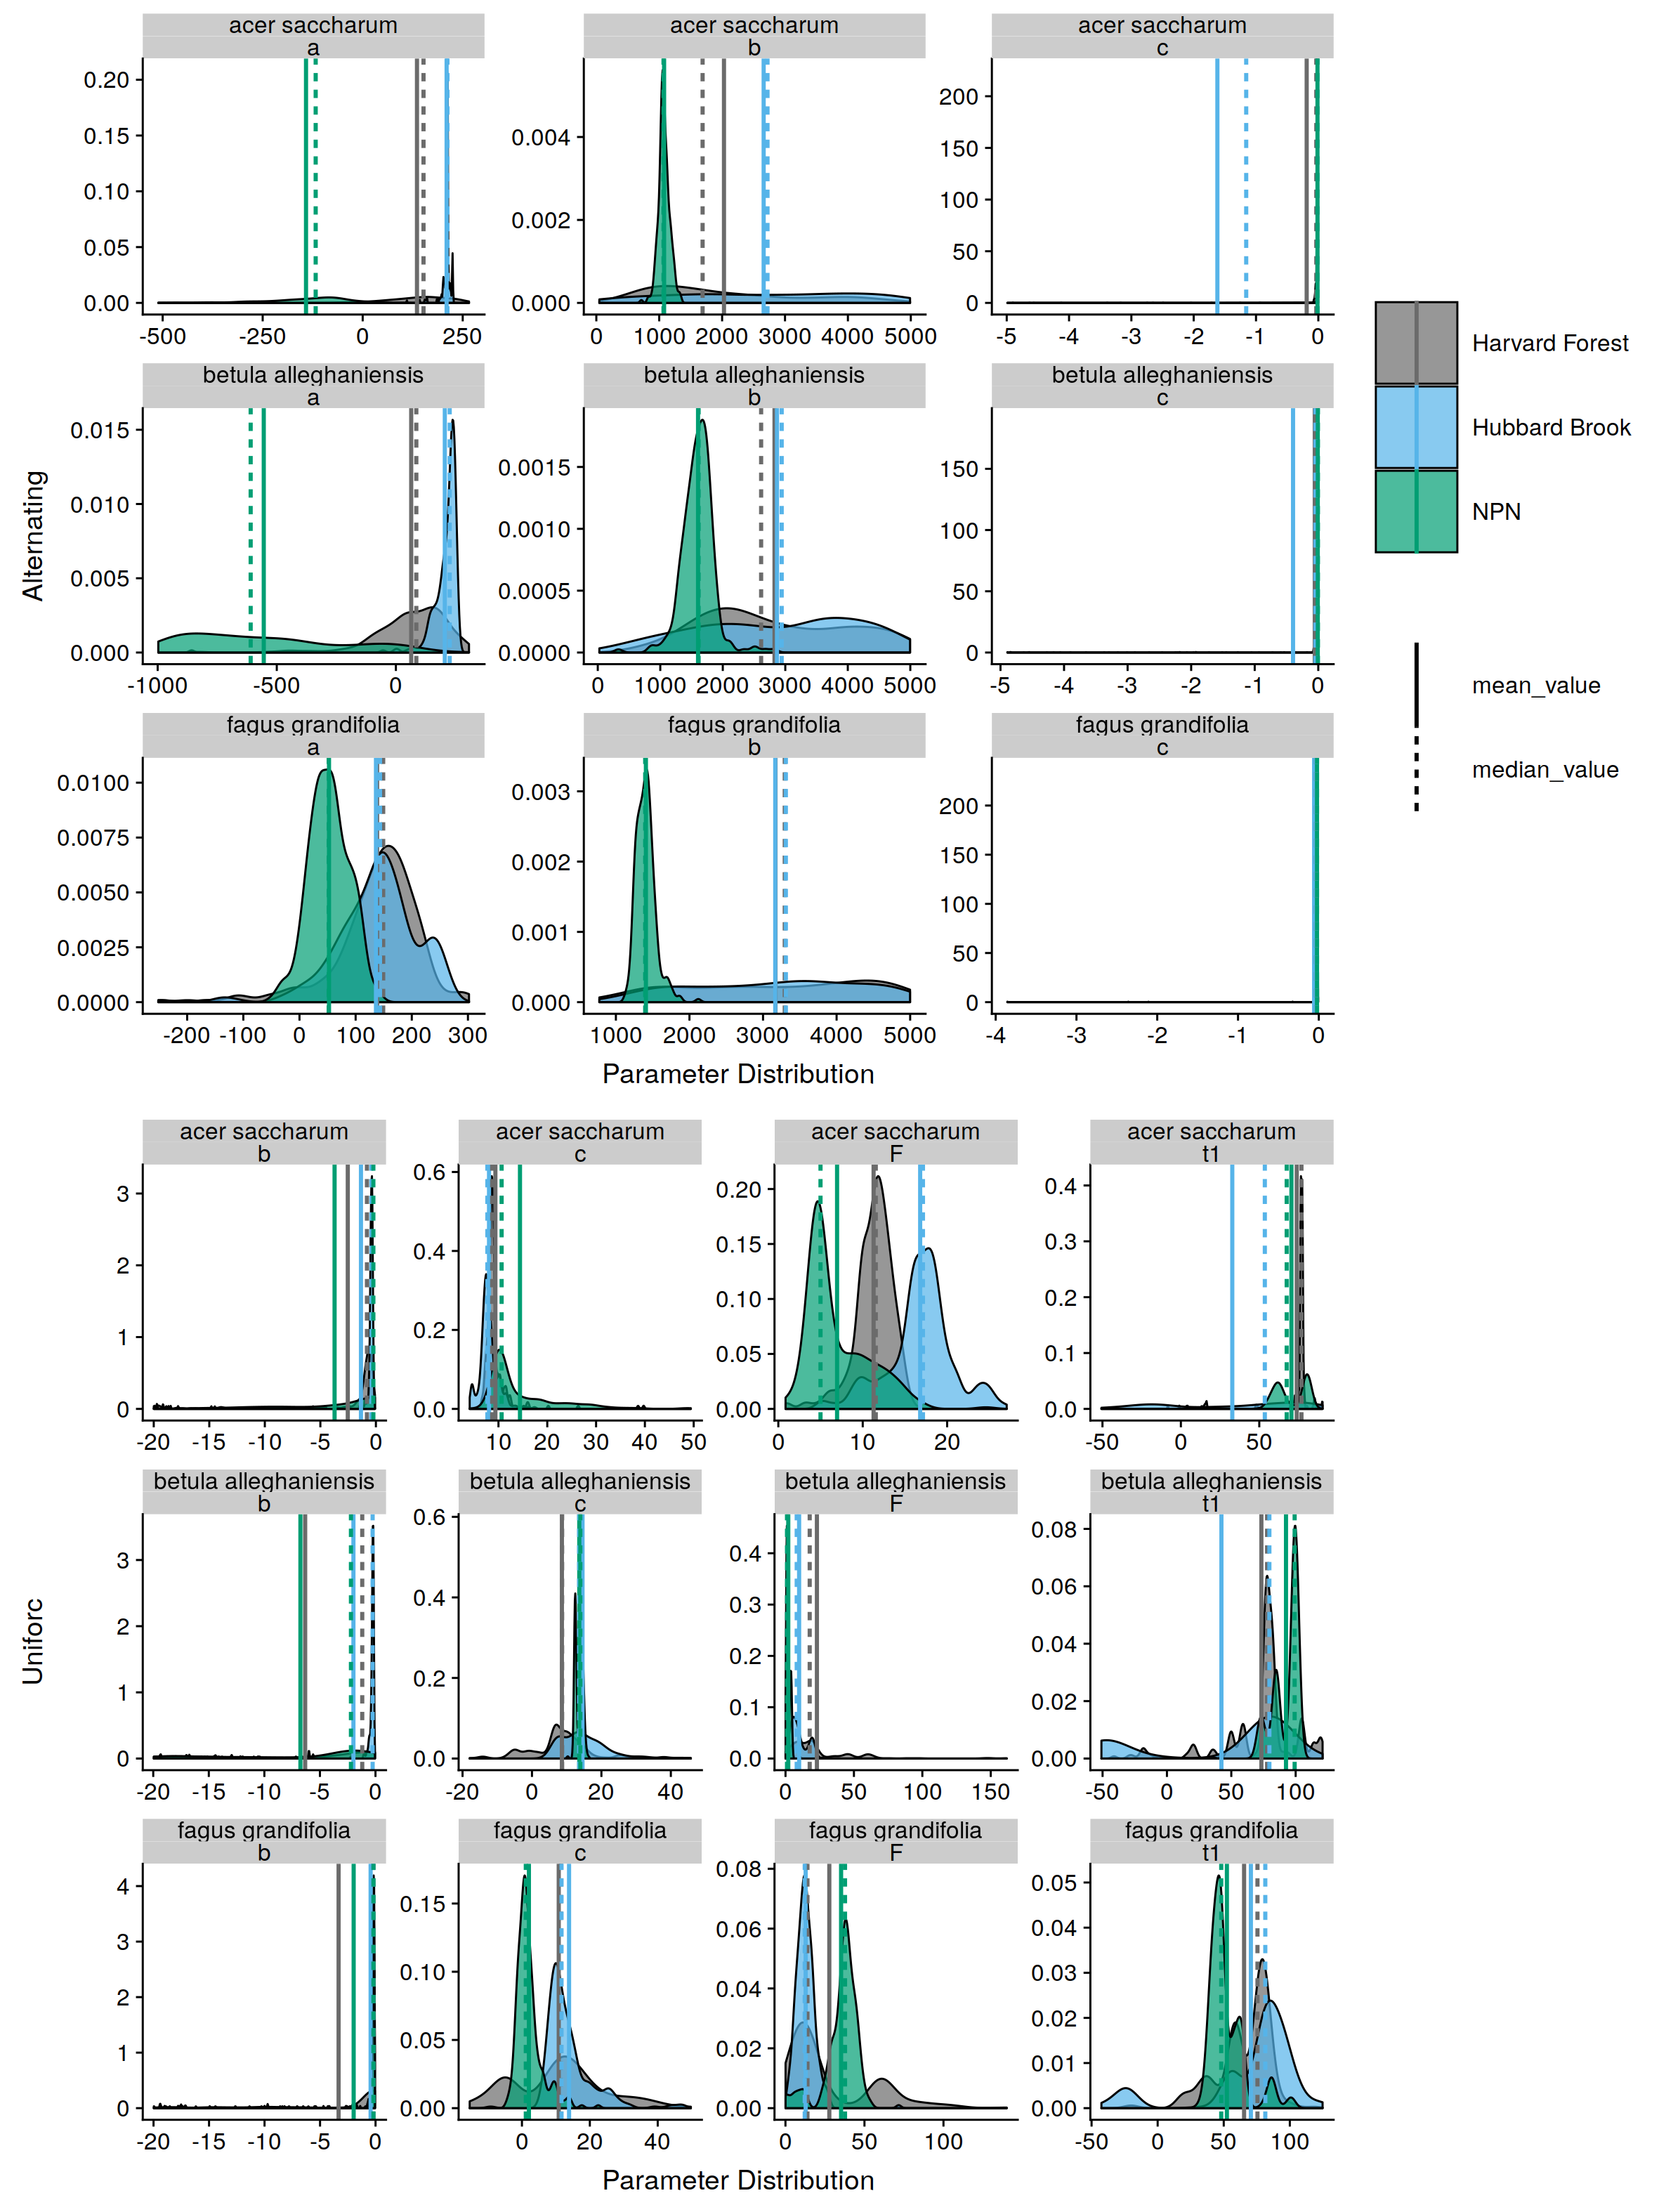
\includegraphics[scale=0.5]{figure_s9_hubbard_harvard_comparison2.png}
	Figure S9
\end{center}

%%%%%%%%%%%%%%%%%
%% Figure S10
%%%%%%%%%%%%%%%%%
\newpage

\textbf{Figure S10}: As in Figure S4, but for 4 selected species to show the difference in parameter distributions between LTER and USA-NPN derived models. The phenophase for the four species is budburst. These 4 species are representative of the analysis, and for the remaining comparisons the reader is pointed to the script 'analysis/plot\_select\_species\_parameters.R' in the code repository to generate additional figures.

\newpage

\begin{center}
	\centering
		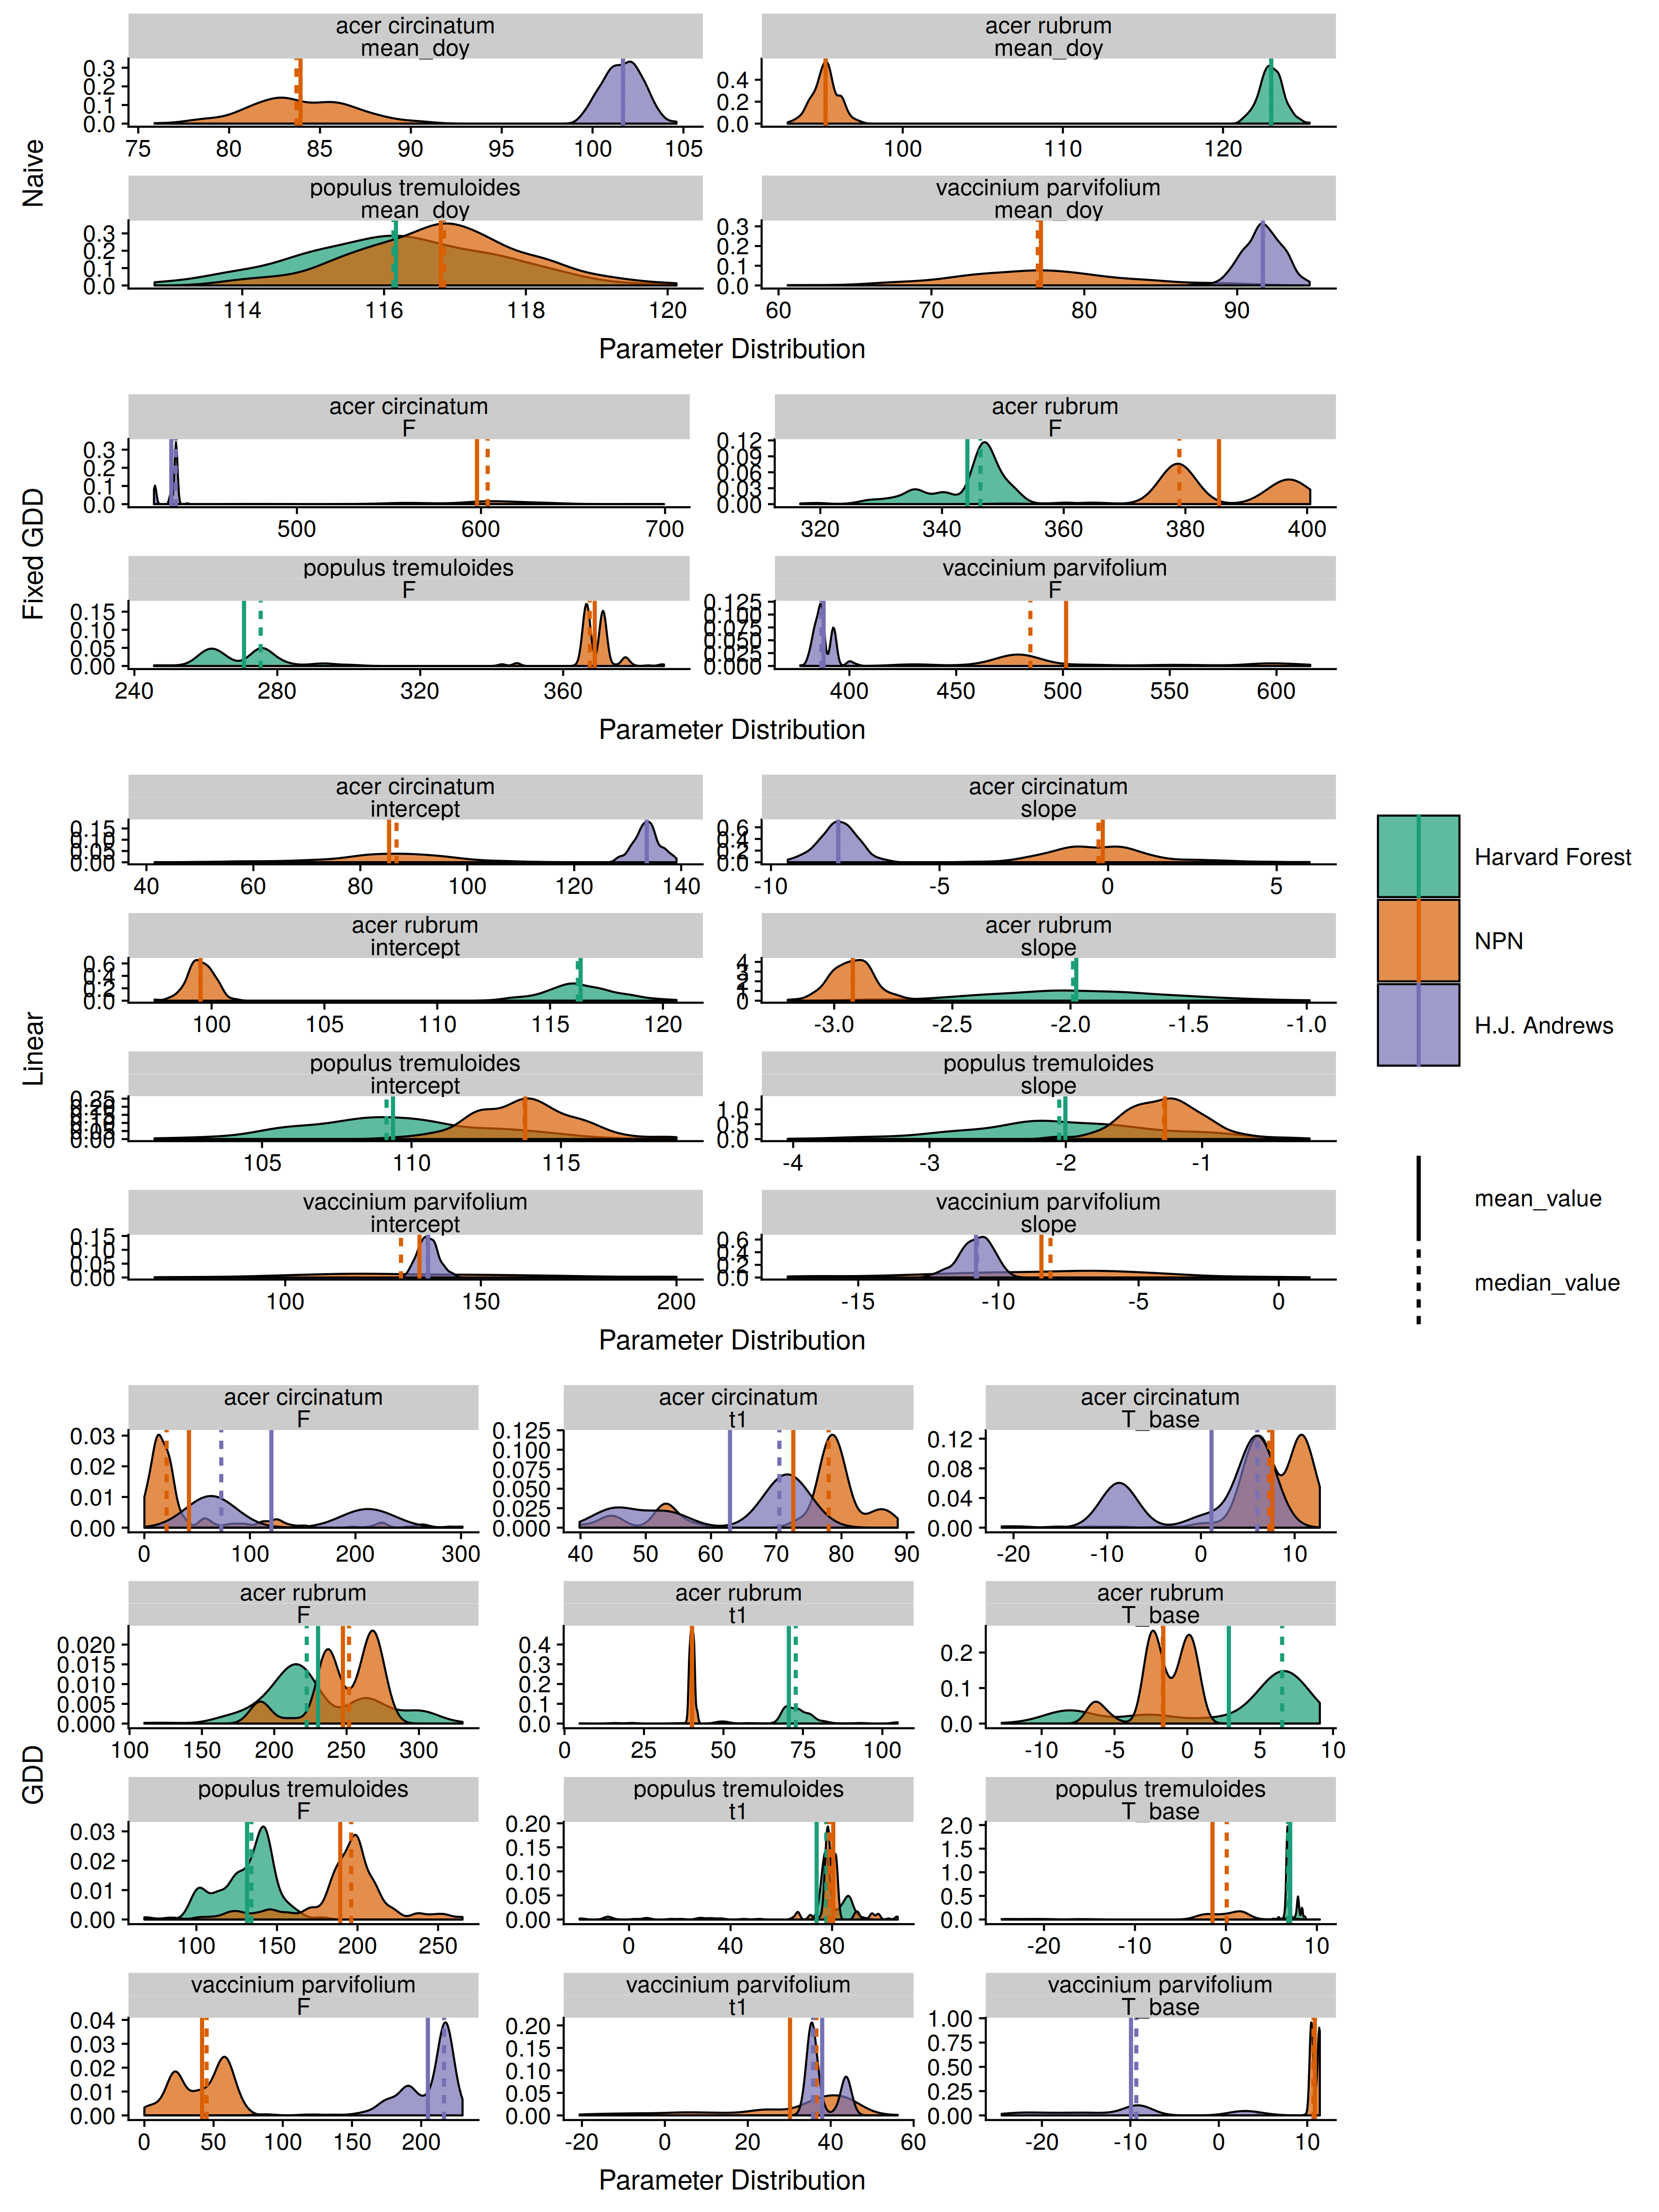
\includegraphics[scale=0.5]{figure_s10_select_species_param_comparison1.png}
	Figure S10
\end{center}

%%%%%%%%%%%%%%%%%
%% Figure S11
%%%%%%%%%%%%%%%%%
\newpage

\textbf{Figure S11}: As in Figure S6, but for the Alternating and Uniforc models. 

\newpage

\begin{center}
	\centering
		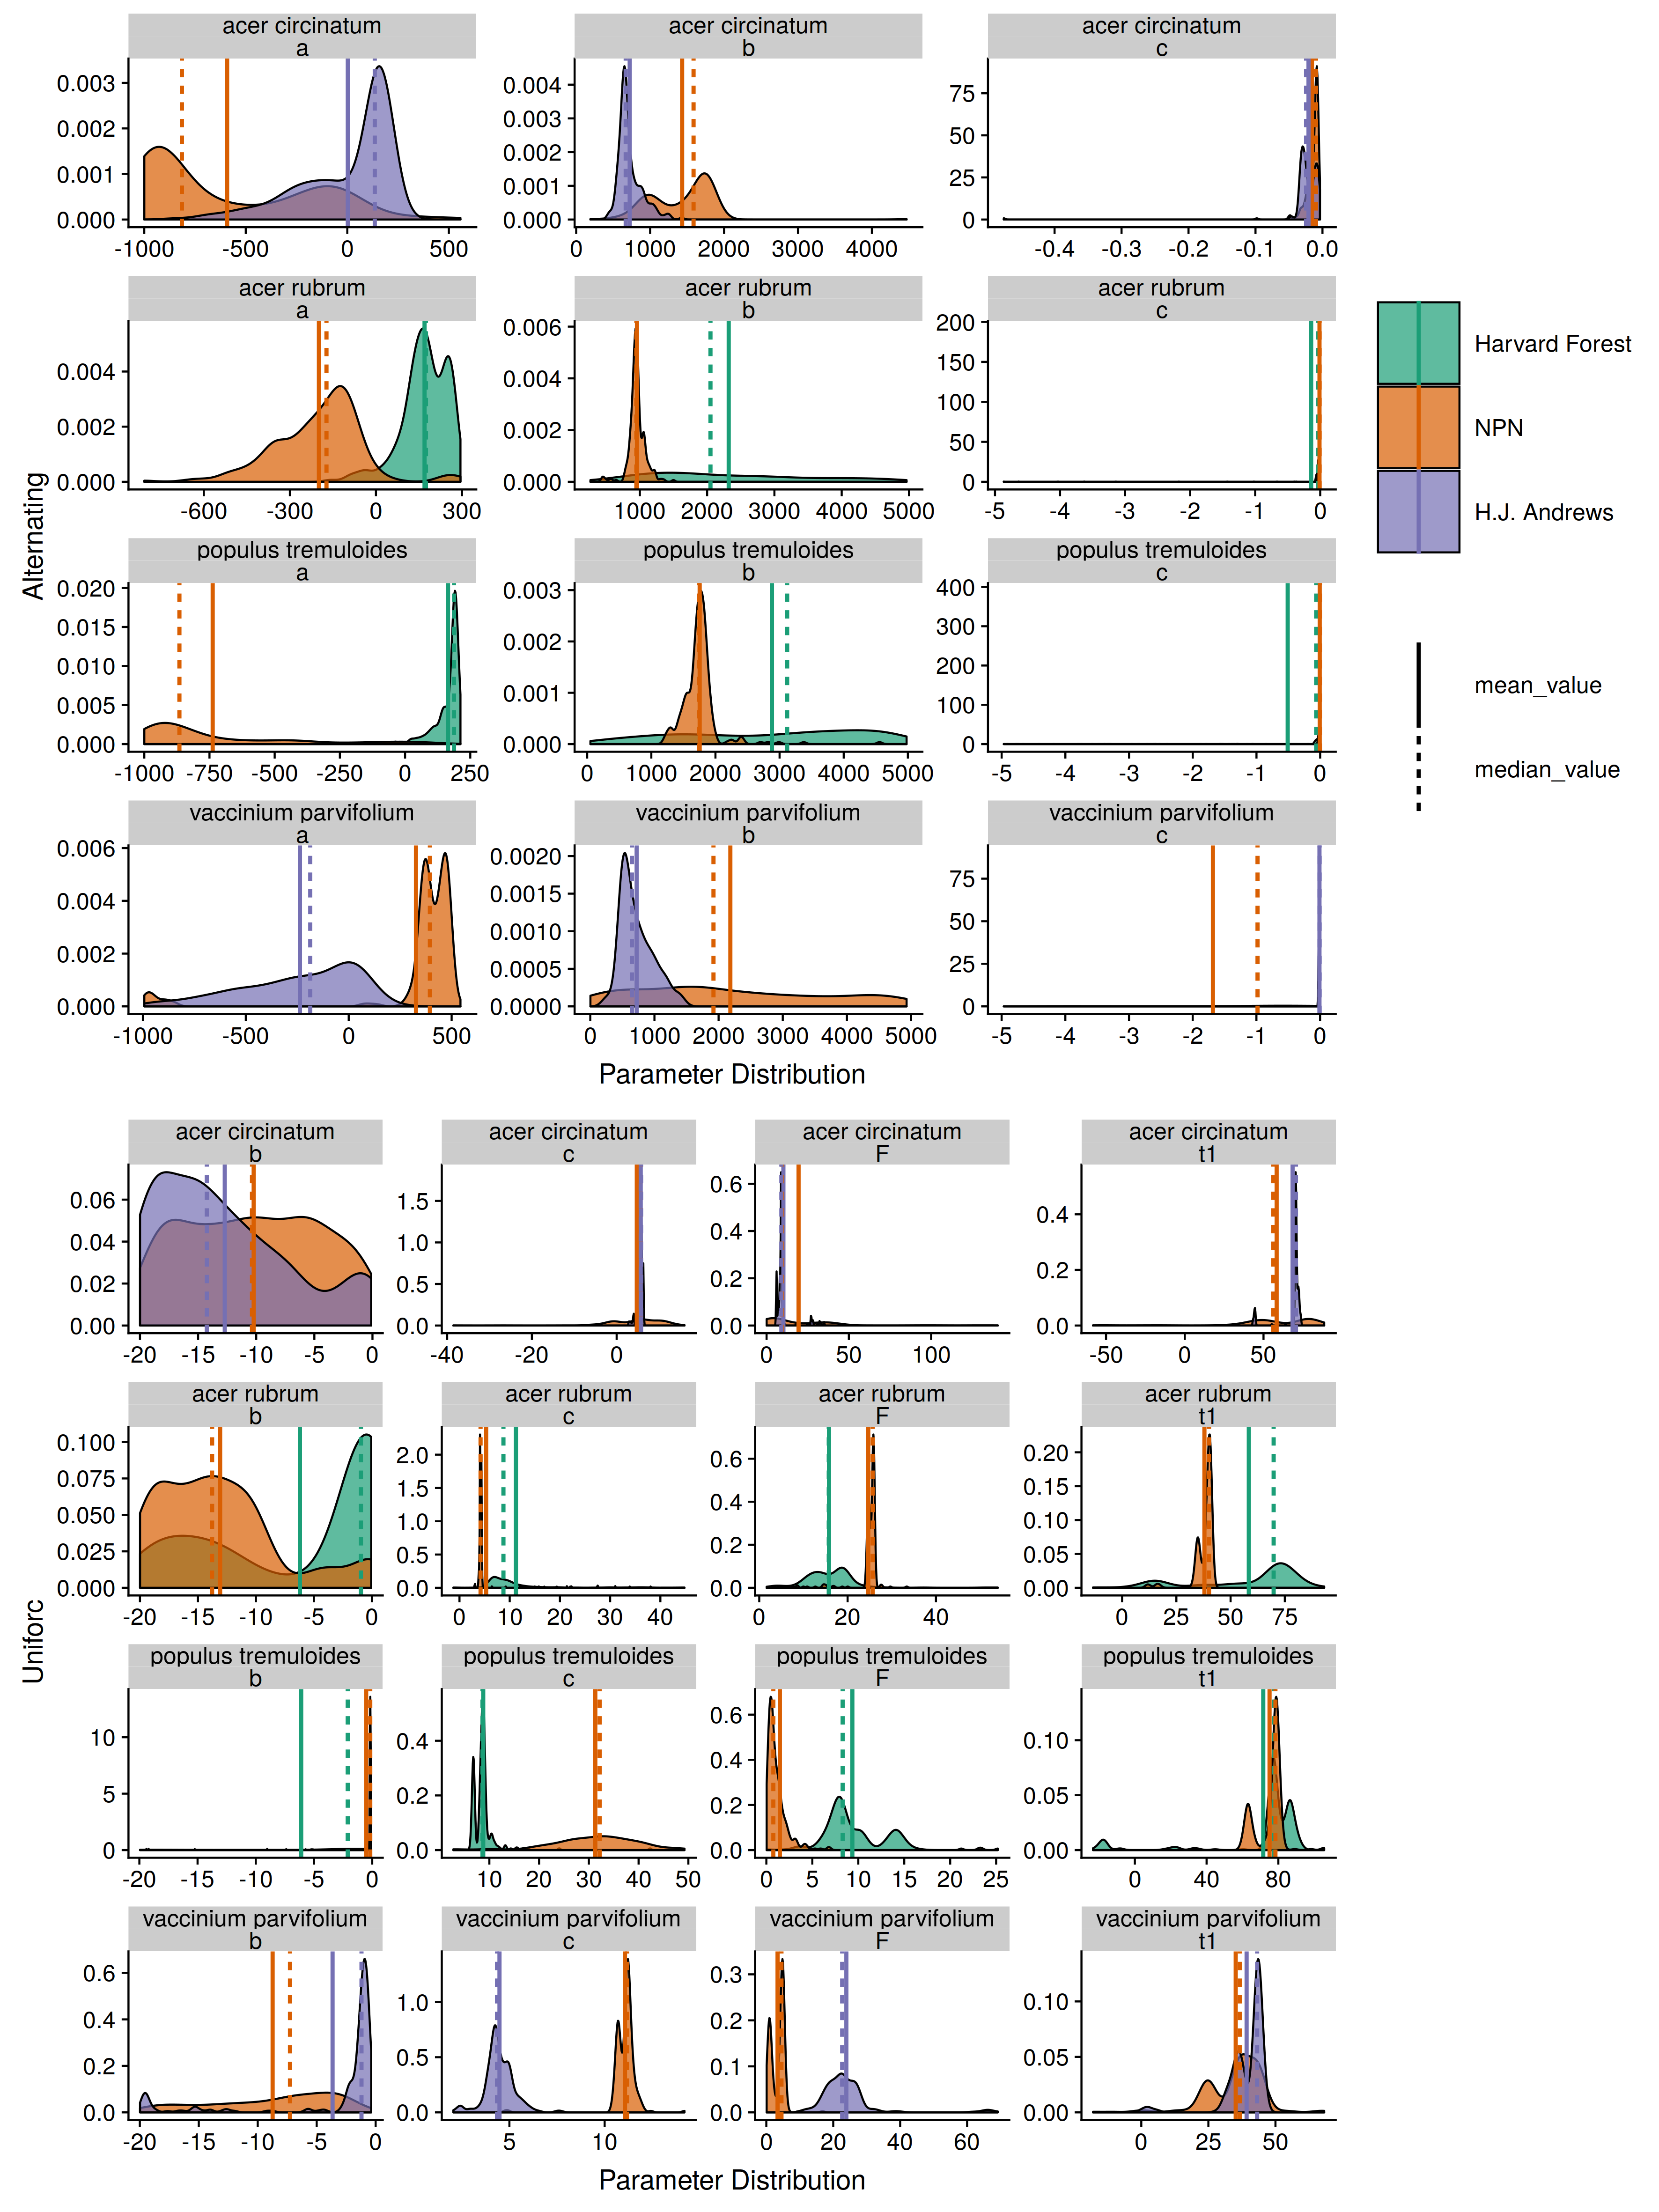
\includegraphics[scale=0.5]{figure_s11_select_species_param_comparison2.png}
	Figure S11
\end{center}
%%%%%%%%%%%%%%%%%
%% Table S1
%%%%%%%%%%%%%%%%%
\newpage

\textbf{Table S1}: Species used in the analysis along with the sample size from each dataset. The numbers indicate the sample size of the training data and the size of the testing data in parenthesis. 

\newpage

\tiny
\begin{tabular}{l|r|l|l|l|l|l|l}
\hline
species & phenophase & phenophase\_type & harvard & hjandrews & hubbard & jornada & npn\\
\hline
acer circinatum & 371 & Budburst & - & 266 (66) & - & - & 39 (10)\\
\hline
acer circinatum & 501 & Flowers & - & 116 (29) & - & - & 33 (8)\\
\hline
acer pensylvanicum & 371 & Budburst & 80 (20) & - & - & - & 34 (9)\\
\hline
acer rubrum & 371 & Budburst & 100 (25) & - & - & - & 957 (239)\\
\hline
acer rubrum & 501 & Flowers & 96 (24) & - & - & - & 668 (167)\\
\hline
acer saccharum & 371 & Budburst & 60 (15) & - & 164 (41) & - & 365 (91)\\
\hline
betula alleghaniensis & 371 & Budburst & 60 (15) & - & 178 (44) & - & 133 (33)\\
\hline
betula alleghaniensis & 501 & Flowers & 26 (7) & - & - & - & 64 (16)\\
\hline
betula lenta & 371 & Budburst & 58 (14) & - & - & - & 96 (24)\\
\hline
betula papyrifera & 371 & Budburst & 76 (19) & - & - & - & 96 (26)\\
\hline
betula papyrifera & 501 & Flowers & 18 (5) & - & - & - & 36 (9)\\
\hline
fagus grandifolia & 371 & Budburst & 76 (19) & - & 177 (44) & - & 259 (65)\\
\hline
fraxinus americana & 371 & Budburst & 84 (21) & - & - & - & 90 (23)\\
\hline
fraxinus americana & 501 & Flowers & 22 (6) & - & - & - & 52 (13)\\
\hline
ilex verticillata & 371 & Budburst & 35 (9) & - & - & - & 26 (6)\\
\hline
larrea tridentata & 501 & Flowers & - & - & - & 27 (7) & 118 (30)\\
\hline
nyssa sylvatica & 371 & Budburst & 27 (7) & - & - & - & 63 (16)\\
\hline
pinus strobus & 496 & Budburst & 38 (10) & - & - & - & 77 (19)\\
\hline
populus tremuloides & 371 & Budburst & 38 (10) & - & - & - & 208 (51)\\
\hline
populus tremuloides & 501 & Flowers & 17 (4) & - & - & - & 79 (22)\\
\hline
prosopis glandulosa & 501 & Flowers & - & - & - & 49 (12) & 78 (20)\\
\hline
prunus serotina & 371 & Budburst & 58 (14) & - & - & - & 228 (57)\\
\hline
pseudotsuga menziesii & 480 & Budburst & - & 182 (46) & - & - & 38 (10)\\
\hline
quercus alba & 371 & Budburst & 62 (15) & - & - & - & 174 (43)\\
\hline
quercus rubra & 371 & Budburst & 80 (20) & - & - & - & 242 (60)\\
\hline
quercus rubra & 501 & Flowers & 56 (14) & - & - & - & 127 (32)\\
\hline
quercus velutina & 371 & Budburst & 77 (19) & - & - & - & 72 (18)\\
\hline
rhododendron macrophyllum & 371 & Budburst & - & 84 (21) & - & - & 48 (12)\\
\hline
rhododendron macrophyllum & 501 & Flowers & - & 27 (7) & - & - & 50 (12)\\
\hline
trillium ovatum & 488 & Budburst & - & 222 (55) & - & - & 68 (17)\\
\hline
trillium ovatum & 501 & Flowers & - & 169 (42) & - & - & 60 (15)\\
\hline
vaccinium corymbosum & 371 & Budburst & 38 (10) & - & - & - & 60 (15)\\
\hline
vaccinium corymbosum & 501 & Flowers & 38 (10) & - & - & - & 65 (16)\\
\hline
vaccinium parvifolium & 371 & Budburst & - & 149 (37) & - & - & 25 (6)\\
\hline
vaccinium parvifolium & 501 & Flowers & - & 162 (41) & - & - & 25 (6)\\
\hline
\end{tabular}
\newline
Table S1 \newline

%%%%%%%%%%%%%%%%%
%% Table S2
%%%%%%%%%%%%%%%%%
\newpage
\normalsize
\textbf{Table S2}: Overall best models when doing cross dataset comparisons. Observations for all species and phenophases were aggregated together to calculate RMSE and Pearsons coefficient for each combination of Parameter source (either USA-NPN or LTER), observation source (either USA-NPN or LTER), and model (6 possible phenology models). Bold indicates the best performing model for a specific parameter and observation combination, with some combinations having ties among multiple models.  

\newpage

\tiny
\begin{adjustbox}{angle=90}
\begin{tabular}{|c|c|cc|cc|cc|cc|cc|cc|cc|cc|}
\hline
\begin{tabular}[c]{@{}c@{}}Parameter\\ Source\end{tabular} & \begin{tabular}[c]{@{}c@{}}Held Out\\ Observation Source\end{tabular} & \multicolumn{2}{c|}{Alternating} & \multicolumn{2}{c|}{Fixed GDD} & \multicolumn{2}{c|}{GDD} & \multicolumn{2}{c|}{Linear} & \multicolumn{2}{c|}{M1} & \multicolumn{2}{c|}{MSB} & \multicolumn{2}{c|}{Naive} & \multicolumn{2}{c|}{Uniforc} \\
 &  & p & RMSE & p & RMSE & p & RMSE & p & RMSE & p & RMSE & p & RMSE & p & RMSE & p & RMSE \\ \hline
LTER & LTER & 0.87 & 8.73 & 0.84 & 10.14 & \textbf{0.90} & 7.89 & 0.81 & 10.27 & \textbf{0.90} & 7.89 & 0.87 & 8.73 & 0.72 & 12.35 & \textbf{0.90} & \textbf{7.86} \\ \hline
LTER & USA-NPN & 0.44 & 26.07 & \textbf{0.72} & 22.70 & 0.68 & 20.52 & 0.65 & 22.94 & 0.68 & 20.52 & 0.44 & 26.07 & 0.34 & 31.25 & 0.70 & \textbf{19.69} \\ \hline
USA-NPN & LTER & 0.63 & 16.17 & 0.69 & 16.15 & 0.70 & 13.73 & 0.68 & 16.59 & 0.71 & 13.79 & 0.66 & 15.79 & 0.61 & 27.08 & \textbf{0.72} & \textbf{13.48} \\ \hline
USA-NPN & USA-NPN & 0.80 & 15.27 & 0.76 & 20.18 & \textbf{0.82} & 14.67 & 0.77 & 16.19 & \textbf{0.82} & 14.71 & 0.80 & 15.20 & 0.53 & 21.57 & \textbf{0.82} & \textbf{14.37} \\ \hline
\end{tabular}
\end{adjustbox}
\newline
Table S2

\end{document}}
